\RequirePackage{kvoptions-patch}
\documentclass[11pt,twoside]{scrartcl}
%\usepackage[ngerman]{babel}
\usepackage[T1]{fontenc}
\usepackage[utf8]{inputenc}
\usepackage{url}
\usepackage{lmodern}
\usepackage{amsmath}
\usepackage{amssymb}
\usepackage{gauss}
\usepackage{graphicx}
\usepackage{pict2e}
\usepackage{curve2e}
\usepackage[scaled=0.75]{luximono}
\usepackage{listings}
\lstset{
	numbers=left,
	numbersep=5pt,
	numberstyle=\tiny,
	language=C++,
	basicstyle=\small\ttfamily,
	keywordstyle=\bfseries,
	frame=shadowbox,
	columns=fullflexible,
	breaklines=true,
	float,
	tabsize=6}
\usepackage[
	title={Development of a FEM code for fluid-structure coupling},
	author={Stephan Herb},
	type=master,
	institute=ipvs,
	number=314159, %TODO Nummer vom Prüfungsamt/-ausschuss erfahren
	course=cs,
	examiner={Prof.\ Dr.\ Miriam Mehl},
	supervisor={Dipl.-Ing.\ Florian Lindner},
	startdate={2015-06-08},
	enddate={2015-12-08},
	crk={}, %TODO CRK-Klassifikation auf meine Arbeit ändern
	language=german
	]{uni-stuttgart-cs-cover}

\begin{document}
\Coverpage
\tableofcontents

\begin{center}
\small{\textbf{Abstract}}
\end{center}

\begin{abstract}
\noindent \small{Dieser Paragraph enthält eine nette kleine Zusammenfassung, in der zusammengefasst ist, was diese Arbeit enthält und tolles neues gemacht hat, das die Welt revolutionieren wird. Dieser Text hier dient im Augenblick nur als Platzhalter und wer ihn liest, sollte sich nicht beklagen, dass er oder sie gerade Zeit verschwendet hat.}
\end{abstract}

\section{Introduction}
Here comes the introduction. And before that the abstract (that needs to be put into \LaTeX as special paragraph)\newpage
% Batoz_et_al-1982 \cite{batoz1982evaluation} hat gute intro an der man schauen kann, wie man eine macht

\section{Framework Evaluation}
Part of the thesis was to find several frameworks which ease the work with the finite element method. An evaluation of these frameworks was done to select a suitable one for the given task. The evaluation's criteria are presented in this chapter as well as a short description of the studied frameworks.
 \subsection{General Aspects}
In preparation of evaluating the frameworks many criteria were created to objectify the search for the most suitable. The individual aspects were as follows:
 \begin{itemize}
 \item Open Source: All frameworks under consideration need to be published under the GNU Lesser General Public License or similar license that allows modification and/or redistribution.
 \item Parallelization: In order to accelerate the calculations the framework has to be able to support the widely used Message Passing Interface (MPI).
 \item The programming language was chosen to be C++. Therefore the framework has to be written in this language. %TODO: warum c++: persönlich größere erfahrung, python wäre generell auch denkbar
 \item Mesh file import: Common mesh files types like gmsh or xda/xdr must be able to load by the framework. Simultaneously the framework must support finite elements like triangles and quadrilaterals with three and four nodes respectively and be able to handle two dimensional elements defined within three dimensional space. %TODO warum muss framework meshes importieren können, was setze ich beim mesh file voraus; es geht auch ein vom framework selbst definiertes format, so lange es die bedingungen erfüllt und einfach reproduzierbar ist
 \item The framework should handle different types of boundary conditions defined in a mesh file. %TODO diesen punkt mit dem vorigen verschmelzen, die bcs sind meine forderungen
 \item Built-in solvers: In order so solve the matrix-vector-system the framework must provide a variety of different iterative solvers. %TODO siehe zwischenvortrag: höhere flexibilität für anwender
 \item Convenience functions: To optimize the calculations the framework should make use of functions to get matrix-vector and matrix-matrix products, transpose matrix or sparse-matrices.
 \item Accessible and detailed documentation: In order to guarantee maintainability and expandability the framework has to have a good documentation itself. %TODO example-codes, dokumentierte klassen und funktionen, mailing-listen und/oder foren zur einfachen verständigung mit den entwicklern
 \item Up-to-date: The framework should be well maintained and actively supported by its developers to ensure a long term compatibility with possible new features of the thesis' code
 \item The framework should be used by at least a few projects. This shows the framework's importance and usability. %TODO nicht nur projects sondern auch publikationen
 \item Easy-to-learn syntax and structure: A rather subjective aspect but an important one. The limited time for the thesis does not allow to study highly complicated structures or semantics. This accompanies the documentation aspect.
 \end{itemize}
 \subsection{Frameworks Overview}
 The following list contains FEM libraries and frameworks which were evaluated.
%  \subsubsection{FEniCS}
  \subsubsection{Feel++}
  - "Feel++ is a unified C++ implementation of Galerkin methods (finite and spectral element methods) in 1D, 2D and 3D to solve partial differential equations."\cite{feelpp}\newline
  - creation of versatile mathematical kernels allow testing and comparing different techniques and methods in solving problems\newline
  - focus on close mathematical abstractions regarding partial differential equations (PDE)\newline
  - \cite{prud2012feel++}
  - imports e.g. gmsh mesh files\newline
  - seamlessly parallel with mpi\newline
  - currently used in projects at Cemosis (Center for Modeling and Simulation in Strasbourg, France) including fluid structure interactions, high field magnets simulation, or, optical tomography\newline
  - actively developed, last major release were on February 2015
  \subsubsection{OOFEM}\cite{oofem}
  - Object Oriented Finite Element Solver (OOFEM) 
  - actively developed with latest release from February 2014\newline
  - object oriented architecture; extensible in terms of new element types, boundary conditions or numerical algorithms\newline
  - modules for structural mechanics, transport problems and fluid dynamics\newline
  - focuses on efficient and robust solution to mechanical, transport and fluid problems\newline
  - written in C++ with focus on portability\newline
  - interfaces to various external software libraries like PETSc, ParMETIS, or, ParaView\newline
  - is used in several publications \cite{oofemPubs}
  \subsubsection{GetFEM++}
  - latest release from July 2015
  - framework for solving potentially coupled systems of linear and nonlinear PDE\newline
  - written in C++ but provides interfaces to languages like Python and Matlab\newline
  - model description that gather the variables, data and terms of a problem and some predefined bricks representing classical models\newline
  - easy switching from one method to another due to separation of geometric transformation, integration methods, and, finite element method\newline
  - can be used to construct generic finite element codes, where methods and the problem's dimension can be changed very easily\newline
  - uses MPI for parallelization, though it is stated that "a certain number of procedures are still remaining sequential" \cite{getfemppMPI}
  - imports e.g. gmsh mesh files\newline
  - used in project like IceTools \cite{icetools} (open source model for glaciers), EChem++ \cite{echempp} (Problem Solving Environment for Electochemistry) and SimNIBS \cite{simnibs} (software for Simulation of Non-invasive Brain Stimulation)
  \subsubsection{MFEM}\cite{mfem}
  - The Modular Finite Element Method (MFEM) library acts as a toolbox that provides the building blocks for developing finite element algorithms\newline
  - it has a wide range of mesh types, e.g. triangular and quadrilateral 2D elements, curved boundary elements or topologically periodic meshes\newline
  - supports MPI-based parallelism throughout the library\newline
  - variety of built-in solvers\newline
  - written in highly portable C++ and extensible due to separation of mesh, finite element and linear algebra abstractions\newline
  - hypre library is tightly integrated within MFEM, for example the use of high-performance preconditioners
  - The object oriented design of the library as well as the separation of the different parts of the library like the mesh functions, the finite elements, and, the linear algebra, focusing on adapt the code to a variety of applications
  - use in several publications \cite{mfemPubs}
  \subsubsection{libMesh}\cite{libmesh}
  - actively developed and active user community\newline
  - wide variety of mesh file formats to import from (e.g. gmsh, vtk, xda, )\newline
  - seamlessly integrated parallel functionality with MPI\newline
  - seamlessly interfaces optional external libraries like PETSc or ParMETIS\newline
  - complete documentation and documented source code available\newline
  - "framework for the numerical simulation of PDE using arbitrary unstructured discretizations on serial and parallel platforms".\newline
  - "provide support for adaptive mesh refinement (AMR) computations in parallel"\newline
  - supports a variety of 1D, 2D, and 3D geometric and finite element types\newline
  - created at The University of Texas at Austin in the CFDLab in March 2002. Contributions have come from developers at the Technische Universität Hamburg-Harburg Institute of Modelling and Computation, CFDLab associates at the PECOS Center at UT-Austin, the Computational Frameworks Group at Idaho National Laboratory, NASA Lyndon B. Johnson Space Center, and MIT.
% \subsection{Comparison}
\newpage

\section{Shell Elements}
Mathematical fundamentals of shell elements divided into the two parts and the coordinate transformation
 \subsection{Introduction to Linear Elasticity Problems}
 - \cite{steinke2005finite} ch3.1 (S.61)\newline
 - Einführung von Vektoren und Matrizen (Verschiebungsvektor, Tensoren bzw. Vektoren der Dehnungen und Spannungen)\newline
 - Verknüpfung der Versch. mit den Dehnungen + Stoffgesetz (kinematische Beziehung)\newline
 - ???
 
 In the following the fundamental equations of linear elasticity will be considered. Here, the spatial case is used for demonstration, but every lower dimensional problem can easily be derived from it.
 The following definitions will be used in this thesis:
 \begin{equation}
 \vec{u}^T = \left(u\ v\ w\right)\ \mathrm{displacement\ vector}
 \end{equation}
 \begin{equation}
 \vec{f}^T = \left(f_x\ f_y\ f_z\right)\ \mathrm{external\ force\ vector}
 \end{equation}
 The strains and stresses can either be described in form of tensors $\underline{\epsilon}$ and $\underline{\sigma}$, or as vectors $\vec{\epsilon}$ and $\vec{\sigma}$:
 \begin{equation}
 \underline{\epsilon} = \begin{pmatrix}
 \epsilon_{xx} & \epsilon_{xy} & \epsilon_{xz} \\
 \epsilon_{yx} & \epsilon_{yy} & \epsilon_{yz} \\
 \epsilon_{zx} & \epsilon_{zy} & \epsilon_{zz} \end{pmatrix};
 \underline{\sigma} = \begin{pmatrix}
 \sigma_{xx} & \sigma_{xy} & \sigma_{xz} \\
 \sigma_{yx} & \sigma_{yy} & \sigma_{yz} \\
 \sigma_{zx} & \sigma_{zy} & \sigma_{zz} \end{pmatrix}
 \end{equation}
 \begin{equation}
 \vec{\epsilon}^T = \begin{pmatrix}
 \epsilon_{xx} & \epsilon_{yy} & \epsilon_{zz} & 2\epsilon_{xy} & 2\epsilon_{yz} & 2\epsilon_{zx} \end{pmatrix};
 \vec{\sigma}^T = \begin{pmatrix}
 \sigma_{xx} & \sigma_{yy} & \sigma_{zz} & \sigma_{xy} & \sigma_{yz} & \sigma_{zx} \end{pmatrix}
 \end{equation}
 As stated in \cite{steinke2005finite} the relation between displacements and strains is as follows:
 \begin{equation}\label{eq:displ_strain_relation}
 \underline{\epsilon} = \frac{1}{2}\left(\nabla\vec{u} + \vec{u}\:\nabla \right);\quad \vec{\epsilon}
 %= \begin{pmatrix}
 %\frac{\partial}{\partial x} & 0 \\
 %0 & \frac{\partial}{\partial y} \\
 %\frac{\partial}{\partial y} & \frac{\partial}{\partial x} \end{pmatrix} \vec{u}
 = \underline{L}\vec{u}
 \end{equation}
 Equation \ref{eq:displ_strain_relation} relates the displacement vector field $\vec{u}$ with the strain field $\underline{\epsilon}$, or $\vec{\epsilon}$ respectively. Here, $\underline{L}$ is a differential operator. This strain-displacement relation is also called \textit{kinematic relationship} \cite{steinke2005finite}.\\
 In general initial strains can exist inside the material for example due to temperature changes or shrinkage. Such initial strains are denoted $\vec{\epsilon_0}$ and the stresses will be influenced by the difference between the actual and initial strains. Additionally one could imagine initial residual stresses $\vec{\sigma_0}$ that can be added to the general equation:
 \begin{equation}\label{eq:stress-strain-relation}
 \vec{\sigma} = \underline{D}\left(\vec{\epsilon}-\vec{\epsilon_0}\right)+\vec{\sigma_0},
 \end{equation}
 where $\underline{D}$ is the material matrix. In the simplest case of linear elasticity with isotropy, $\underline{D}$ only contains two parameters, namely the elastic modulus $E$ (also known as the Young's modulus) and the Poisson's ratio $\nu$. The former one defines the relationship between the stress and strain in a material, the latter one results as the quotient of the fraction of expansion and the fraction of compression for small changes.
 In the following the initial conditions are ignored, resulting in the a simpler form of equation \ref{eq:stress-strain-relation}:
 \begin{equation}
 \vec{\sigma} = \underline{D}\ \vec{\epsilon}
 \end{equation}
 For the said isotropic case $\underline{D}$ results in \cite{zienkiewicz2000finite}:
 \begin{equation}
 \underline{D} = \frac{E}{1-\nu^2}\begin{pmatrix}
 1 & \nu & 0 \\
 \nu & 1 & 0 \\
 0 & 0 & \frac{1-\nu}{2}
 \end{pmatrix}
 \end{equation}
 \subsection{Plane Element}
 First part of shell element: plane part. derivation of this part with two exemplary finite element types
  \subsubsection{Problem Definition}\label{sec:PlaneProbDef}
  %- Bild ähnlich ch7.1 mit xy-Ausdehnung, Dicke t, Mittelfläche, Rand, KoSys; Streckenlast q0 und Volumenkraft g aber weglassen\newline
  \begin{figure}
\centering
\includegraphics[width=0.7\linewidth]{figures/platzhalter}
\caption[kurze Unter-Überschrift]{lange Unter-Überschrift}
\label{fig:platzhalter}
\end{figure}
  In figure \ref{fig:platzhalter} an object is shown which extends to the x and y axis as its primary direction. The extend in z-direction is smaller and denoted by thickness $t$. The mid place located in between the top and bottom surface areas has the coordinate $z=0$. Its local z-axis equals the normal vector of the mid place. Such an object is called \textit{plane} in the following.
  
  %- Bed. für ebenen Spannungszustand (eb. Dehnungszustand erwähnen und auf Ref (z.B. Zienkiewicz) verweisen)\newline
  There are two different problem definitions regarding plane elements: Plane stress and plane strain. The directions of displacements $u$ and $v$ along the orthogonal local x and y axis defining its displacement field is a common feature of both problems. Also, both have in common, that only strains and stresses in the xy plane have to be considered: Instead of nine, only three components remain. While in the case of plane stress all other stress components are zero, in plane strain the stress in direction perpendicular to the xy plane is non-zero. In this thesis only plane stress will be discussed in further detail. More information about plane strain is given in \cite{zienkiewicz2000finite}. %TODO weitere referenz mit details dazu
  The following conditions must be satisfied such that a plane can be in \textit{plane stress} \cite{steinke2005finite}:
  \begin{itemize}
  	\item The thickness $t$ varies only slightly and it must hold: $t/l \ll 1$, with $l$ the extent of the larger side of the plane element.
  	\item The load is applied to the mid place.
  	\item Displacements, strains and stresses are constant across the thickness.
  \end{itemize}
  The stress components $\sigma_{xz},\sigma_{yz},\sigma_{zz}$ normal to the surface areas with $z \pm t/2$ vanish (equals zero). Therefore only the two normal stress components $\sigma_{xx}$ and $\sigma_{yy}$ and the transverse stress component $\sigma_{xy}$ are left non-zero.
    
  %- Verschiebungen, Dehnungen und Spannungen beschreiben + kinematische Beziehung + Stoffgleichung\newline
  Displacements can only occur in x and y direction. $u$ will be the displacement along x and $v$ along y. The displacement field $\vec{u}$ is as follows:
  \begin{equation}
  \vec{u}=\begin{pmatrix}
  u(x,y) & v(x,y)
  \end{pmatrix}^T
  \end{equation}
  The vector for the strain components:
  \begin{equation}
  \vec{\epsilon}=\begin{pmatrix}
  \epsilon_{xx} & \epsilon_{yy} & 2\epsilon_{xy}
  \end{pmatrix}^T
  \end{equation}
  Sometimes $2\epsilon_{xy}$ is shortened to $\gamma_{xy}$ \cite{steinke2005finite}.
  The vector holding the stress components is similar to that of the strain's vector:
  \begin{equation}
  \vec{\sigma}=\begin{pmatrix}
  \sigma_{xx} & \sigma_{yy} & \sigma_{xy}
  \end{pmatrix}^T
  \end{equation}
  The kinematic relationship $\vec{\epsilon}=\underline{L}\vec{u}$ \ref{eq:displ_strain_relation} linking the displacements $\vec{u}$ with the strains $\vec{\epsilon}$ at full length:
  \begin{equation}\label{eq:t3displ-str-rel}
  \vec{\epsilon} = \begin{pmatrix}
  \epsilon_{xx} \\
  \epsilon_{yy} \\
  2\epsilon_{xy}
  \end{pmatrix} =
  \begin{pmatrix}
  \frac{\partial u}{\partial x} \\
  \frac{\partial v}{\partial y} \\
  \frac{\partial u}{\partial y} + \frac{\partial v}{\partial x}
  \end{pmatrix} =
  \begin{pmatrix}
  \frac{\partial}{\partial x} & 0 \\
  0 & \frac{\partial}{\partial y} \\
  \frac{\partial}{\partial y} & \frac{\partial}{\partial x}
  \end{pmatrix}
  \begin{pmatrix}
  u \\
  v
  \end{pmatrix}
  = \underline{L} \vec{u}
  \end{equation}
  With the strains known and considering equation \ref{eq:displ_strain_relation} one can calculate the stresses $\vec{\sigma}$:
  \begin{equation}\label{eq:sigma=D*eps}
  \vec{\sigma} = \begin{pmatrix}
  \sigma_{xx} \\
  \sigma_{yy} \\
  \sigma_{xy}
  \end{pmatrix} = \frac{E}{1-\nu^2} \begin{pmatrix}
  1 & \nu & 0 \\
  \nu & 1 & 0 \\
  0 & 0 & \frac{1-\nu}{2}
  \end{pmatrix} \begin{pmatrix}
  \epsilon_{xx} \\
  \epsilon_{yy} \\
  2\epsilon_{xy}
  \end{pmatrix} = \underline{D} \vec{\epsilon} = \underline{D}\; \underline{L} \vec{u}
  \end{equation}
  %- Randbedingungen: q0 Streckenlast beschreiben, aber angeben, dass sie hier nicht beachtet werden, punktf. Ladungen werden hier benutzt\newline
  % TODO hier fehlt der Abschnitt über die Randbedingungen steinke s. 214(227)
  natural boundary conditions in form of nodal forces: $\vec{F} = \begin{pmatrix}
  F_x & F_y
  \end{pmatrix}^T$
  
  %- resultierendes Gesamtpotential ohne b und q
  % TODO pi-potenzial einführen
  The total potential of the plane element problem looks as follows:
  \begin{equation}\label{eq:planeFunctional}
  \Pi = 1/2 \int_{V}\vec{\epsilon}^T\vec{\sigma}dV - \vec{u}^T \vec{F},
  \end{equation}
  with the first term being the elastic strain energy and the second term the single forces.
  
  \subsubsection{Tri-3 Plane Element}
  mathematical derivation of three node triangular plane element \textbf{discretization}\\
  see Steinke \cite{steinke2005finite} page 215-221\\
  % Bild von trianguliertem Körper\\
  \begin{figure}
  	\centering
  	\includegraphics[width=0.7\linewidth]{figures/platzhalter}
  	\caption[kurze Unter-Überschrift]{lange Unter-Überschrift}
  	\label{fig:platzhalter}
  \end{figure}
  In section \ref{sec:PlaneProbDef} the plane's functional was derived. Now the focus is on the functional's discretization. Figure \ref{fig:platzhalter} shows a general, planar object defined to be placed in the xy-plane. The first discretization step is to divide the object into single triangles approximating the shape of it. This process is called triangulation. Every one of these triangles then represents a finite element with one node at every corner. The finer the triangulation is done the better the object and its boundary are matched by its discrete complement, but also the more finite elements have to be considered in later calculations.
  \begin{figure}
  	\centering
  	\includegraphics[width=0.7\linewidth]{figures/platzhalter}
  	\caption[kurze Unter-Überschrift]{lange Unter-Überschrift}
  	\label{fig:platzhalter}
  \end{figure}
  One triangular finite element is shown in Figure \ref{fig:platzhalter}. It is defined by the coordinates $(x_i,y_i)$ of its three nodes. Since the element is located in the xy-plane, the z-coordinate is of no interest and will be ignored. At every node, forces can be applied denoted with $F_{x_i}$ and $F_{y_i}$. Accordingly, every node can be displaced. The movement along the x-axis is denoted with $u_i$, or with $v_i$ along the y-axis respectively. Note, that the node numbering is in counter-clockwise direction. This definition will be kept throughout the thesis, and is important to remember when implementing the FEM-code in order to reduce errors.
  In this thesis only triangles defined by three nodes are discussed. There are many more finite elements forming triangles, such as six node triangles or even seven node triangles. The main difference between these types of elements are the order of shape functions. More details about higher order triangular finite elements can be found in %TODO \cite
  
  % ansatzfunktion (abgewandelt statt phi, u und v separat)\\
  In the case of a three node triangle the basis functions for the two displacements $u$ and $v$ are as follows \cite{steinke2005finite}:
  \begin{equation}\label{eq:t3_ansatzU}
  u(x,y) = a_0 + a_1L_1 + a_2L_2 = \begin{pmatrix}
  1 & L_1 & L_2
  \end{pmatrix} \begin{pmatrix}
  a_0 \\ a_1 \\ a_2
  \end{pmatrix} = \vec{x}^T \vec{a},
  \end{equation}
  \begin{equation}\label{eq:t3_ansatzV}
  v(x,y) = a_0 + a_1L_1 + a_2L_2 = \begin{pmatrix}
  1 & L_1 & L_2
  \end{pmatrix} \begin{pmatrix}
  a_0 \\ a_1 \\ a_2
  \end{pmatrix} = \vec{x}^T \vec{a},
  \end{equation}
  both defined in triangular coordinates (see figure \ref{fig:platzhalter}).
  % dreieckskoordinaten (ähnlich bild 2.7 auf s.39(53))
  \begin{figure}
  	\centering
  	\includegraphics[width=0.7\linewidth]{figures/platzhalter}
  	\caption[kurze Unter-Überschrift]{lange Unter-Überschrift}
  	\label{fig:platzhalter}
  \end{figure}
  % interpolationsbedingunen führen auf Formfunktionen\\
  To get the unknown coefficients $a_i$, values for the triangular coordinates are set. This creates a system of linear equations:
  \begin{align}
  u(L_1=1, L_2=0) = u_1 &\rightarrow u_1 = a_0 + a_1 \nonumber\\
  u(L_1=0, L_2=1) = u_2 &\rightarrow u_2 = a_0 + a_2 \nonumber\\
  u(L_1=0, L_2=0) = u_3 &\rightarrow u_3 = a_0
  \end{align}
  Alternatively, this could be also done with $v$. Written as matrix and vector:
  \begin{align}
  \underline{A} \vec{a} = \vec{u} \nonumber\\
  \begin{pmatrix}
  1 & 1 & 0\\
  1 & 0 & 1\\
  1 & 0 & 0
  \end{pmatrix} \begin{pmatrix}
  a_0 \\ a_1 \\ a_2
  \end{pmatrix} = \begin{pmatrix}
  u_1 \\ u_2 \\ u_3
  \end{pmatrix}
  \end{align}
  Now, inverting matrix $A$ the coefficients can be found:
  \begin{equation}\label{eq:t3_coeffsA}
  \vec{a} = \underline{A}^{-1} \vec{u} = \begin{pmatrix}
  0 & 0 & 1\\
  1 & 0 & -1\\
  0 & 1 & -1
  \end{pmatrix} \begin{pmatrix}
  u_1 \\ u_2 \\ u_3
  \end{pmatrix}
  \end{equation}
  If one put equation \ref{eq:t3_coeffsA} into \ref{eq:t3_ansatzU}, or the analogon into \ref{eq:t3_ansatzV}, the shape functions for the three node triangular finite element will be derived, as described in \cite{steinke2005finite}:
  \begin{align}\label{eq:t3SF}
  u &= \vec{x}^T \vec{a} = \vec{x}^T \underline{A}^{-1}\vec{u} = \vec{N}^T\vec{u} \nonumber\\
  \vec{N}^T &= \vec{x}^T \underline{A}^{-1} =
  \begin{pmatrix}
  1 & L_1 & L_2
  \end{pmatrix} \begin{pmatrix}
  0 & 0 & 1\\
  1 & 0 & -1\\
  0 & 1 & -1
  \end{pmatrix} \nonumber\\
  &= \begin{pmatrix}
  L_1 & L_2 & 1-L_1-L_2
  \end{pmatrix} = \begin{pmatrix}
  N_1 & N_2 & N_3
  \end{pmatrix}
  \end{align}
  Characteristically for the shape function, as stated in \cite{steinke2005finite}, is, that shape function $N_i$ gets the value 1 at node $i$ and 0 at the two other nodes. The functions are linear with respect to $L_1$ and $L_2$ which can be noticed in equation \ref{eq:t3SF}. As stated before, these shape functions are the same for displacement $u$ and $v$. With the knowledge of the displacement values of the element's nodes one can formulate the displacement functions in triangular coordinate notation as follows:
  \begin{align}
  u &= N_1 u_1 + N_2 u_2 + N_3 u_3 \nonumber\\
  v &= N_1 v_1 + N_2 v_2 + N_3 v_3
  \end{align}
  Or in matrix form:
  \begin{align} \label{eq:t3u=Nu}
  \vec{\tilde{u}} &= \underline{N} \vec{u} \nonumber\\
  \begin{pmatrix}
  u \\ v
  \end{pmatrix} &= \begin{pmatrix}
  N_1 & 0 & N_2 & 0 & N_3 & 0 \\
  0 & N_1 & 0 & N_2 & 0 & N_3
  \end{pmatrix} \begin{pmatrix}
  u_1 \\ v_1 \\ u_2 \\ v_2 \\ u_3 \\ v_3
  \end{pmatrix}
  \end{align}
  The vector $\vec{\tilde{u}}$ describes the element's displacements as product of matrix $\underline{N}$ containing the shape functions and vector $\vec{u}$ containing the displacements of the single triangle's nodes. Now, one can put equation \ref{eq:t3u=Nu} into \ref{eq:t3displ-str-rel}:
  \begin{equation}\label{eq:t3eps=Bu}
  \vec{\epsilon} = \underline{L}\vec{\tilde{u}} = \underline{L}\;\underline{N} \vec{u} = \underline{B} \vec{u}
  \end{equation}
  The product of $\underline{L}$ and $\underline{N}$ is called \textit{strain-displacement matrix} $\underline{B}$.
  In order to calculate the strain-displacement matrix, one has to assemble the $\underline{L}$ matrix containing the first partial derivatives of the triangular element. With the chain rule applied, the partial derivatives look as follows:
  \begin{align}
  \frac{\partial}{\partial L_1} = \frac{\partial x}{\partial L_1} \frac{\partial}{\partial x} + \frac{\partial y}{\partial L_1} \frac{\partial}{\partial y} \nonumber\\
  \frac{\partial}{\partial L_2} = \frac{\partial x}{\partial L_2} \frac{\partial}{\partial x} + \frac{\partial y}{\partial L_2} \frac{\partial}{\partial y}
  \end{align}
  or in matrix notation:
  \begin{align}\label{eq:t3NablaTilde}
  \tilde{\nabla} &= \underline{J} \nabla \nonumber\\
  \begin{pmatrix}
  \frac{\partial}{\partial L_1}\\ \frac{\partial}{\partial L_2}
  \end{pmatrix} &= \begin{pmatrix}
  \frac{\partial x}{\partial L_1} & \frac{\partial y}{\partial L_1}\\
  \frac{\partial x}{\partial L_2} & \frac{\partial y}{\partial L_2}
  \end{pmatrix} \begin{pmatrix}
  \frac{\partial}{\partial x}\\ \frac{\partial}{\partial y}
  \end{pmatrix},
  \end{align}
  where $\underline{J}$ represents the Jacobian, $\nabla$ the partial derivatives in Cartesian coordinates and $\tilde{\nabla}$ the partial derivatives in triangular coordinates. To get the derivatives in Cartesian form the upper equation must be multiplied with the inverse Jacobian $\underline{J}^{-1}$:
  \begin{equation}
  \underline{J}^{-1} = \frac{1}{|\underline{J}|} \begin{pmatrix}
  \frac{\partial y}{\partial L_2} & -\frac{\partial y}{\partial L_1} \\
  \frac{-\partial x}{\partial L_2} & \frac{\partial x}{\partial L_1}
  \end{pmatrix}
  \end{equation}
  The conversion between triangular and Cartesian coordinates can be summarized as follows (see Figure \ref{fig:platzhalter} and \cite{steinke2005finite}):
  \begin{align}\label{eq:triCoord<->CartCoord}
  L_1 + L_2 + L_3 &= 1 \rightarrow L_3 = 1-L_1-L_2 \nonumber\\
  x &= x_1L_1 + x_2L_2 + x_3L_3 = (x_1-x_3)L_1 + (x_2-x_3)L2 + x_3\\
  y &= y_1L_1 + y_2L_2 + y_3L_3 = (y_1-y_3)L_1 + (y_2-y_3)L2 + y_3 \nonumber
  \end{align}
  Considering equation \ref{eq:triCoord<->CartCoord} the Jacobian can now be calculated
  \begin{equation}
  J = \begin{pmatrix}
  \frac{\partial x}{\partial L_1} = x_1-x_3 = x_{13} & \frac{\partial y}{\partial L_1} = y_1-y_3 = y_{13}\\
  \frac{\partial x}{\partial L_2} = x_2-x_3 = x_{23} & \frac{\partial y}{\partial L_2} = y_2-y_3 = y_{23}
  \end{pmatrix} = \begin{pmatrix}
  x_{13} & y_{13}\\
  x_{23} & y_{23}
  \end{pmatrix}
  \end{equation}
  and hence the inverse Jacobian:
  \begin{equation}\label{eq:t3invJac}
  \underline{J}^{-1} = \frac{1}{2 A_\triangle} \begin{pmatrix}
  y_{23} & -y_{13}\\
  -x_{23} & x_{13}
  \end{pmatrix}
  \end{equation}
  The determinant of the Jacobian is two times the area of the triangle. With the help of equation \ref{eq:t3invJac}, \ref{eq:t3NablaTilde} can be reorganized
  \begin{equation}
  \nabla = \underline{J}^{-1} \tilde{\nabla}
  \end{equation}
  and this finally yields to the new version of the differential operator $\underline{L}$ \cite{steinke2005finite}:
  \begin{align}
  \underline{L} = \frac{1}{2 A_\triangle} \begin{pmatrix}
  y_{23}\frac{\partial}{\partial L_1} - y_{13}\frac{\partial}{\partial L_2} & 0 \\
  0 & -x_{23}\frac{\partial}{\partial L_1} + x_{13}\frac{\partial}{\partial L_2} \\
  -x_{23}\frac{\partial}{\partial L_1} + x_{13}\frac{\partial}{\partial L_2} & y_{23}\frac{\partial}{\partial L_1} - y_{13}\frac{\partial}{\partial L_2}
  \end{pmatrix}
  \end{align}
  
  % Dehnungs-Verschiebungs-Beziehung -> führt zu B + Spannungs-Verschiebungs-Beziehung\\
  Next, the strain-displacement matrix $\underline{B}$ can be calculated:
  \begin{align}
  \underline{B} &= \underline{L}\; \underline{N} \nonumber\\
  &= \frac{1}{2 A_\triangle} \begin{pmatrix}
  y_{23}\frac{\partial}{\partial L_1} - y_{13}\frac{\partial}{\partial L_2} & 0 \\
  0 & -x_{23}\frac{\partial}{\partial L_1} + x_{13}\frac{\partial}{\partial L_2} \\
  -x_{23}\frac{\partial}{\partial L_1} + x_{13}\frac{\partial}{\partial L_2} & y_{23}\frac{\partial}{\partial L_1} - y_{13}\frac{\partial}{\partial L_2}
  \end{pmatrix} \nonumber\\
  & \quad \begin{pmatrix}
  L_1 & 0 & L_2 & 0 & 1-L_1-L_2 & 0 \\
  0 & L_1 & 0 & L_2 & 0 & 1-L_1-L_2
  \end{pmatrix} \nonumber\\
  &= \frac{1}{2 A_\triangle} \begin{pmatrix}
  y_{23} & 0 & -y_{13} & 0 & y_{12} & 0 \\
  0 & -x_{23} & 0 & x_{13} & 0 & -x_{12} \\
  -x_{23} & y_{23} & x_{13} & -y_{13} & -x_{12} & y_{12}
  \end{pmatrix}
  \end{align}
  
  % Einsetzen in Gesamtpotential + Variation\\
  With $\underline{B}$ known, one can insert equation \ref{eq:t3eps=Bu} into \ref{eq:sigma=D*eps} to get the stresses:
  \begin{equation} \label{eq:t3sigma=DBu}
  \vec{\sigma} = \underline{D}\;\underline{B} \vec{u}
  \end{equation}
  Finally, every term of the plane element's functional \ref{eq:planeFunctional} can be filled with the above discretized terms:
  \begin{align}\label{eq:t3functional}
  \Pi &= \frac{1}{2} \int_{V}\vec{\epsilon}^T\vec{\sigma}\;dV - \vec{u}^T \vec{F} \nonumber\\
      &= \frac{1}{2} \int_{V}\vec{u}^T \underline{B}^T\underline{D}\;\underline{B}\vec{u}\;dV - \vec{u}^T \vec{F} \nonumber\\
      &= \frac{1}{2} \vec{u}^T \int_{V} \underline{B}^T\underline{D}\;\underline{B}\;dV \vec{u}- \vec{u}^T \vec{F} \nonumber\\
      &= \frac{1}{2}\vec{u}^T \underline{K} \vec{u} - \vec{u}^T \vec{F}
  \end{align}
  with $\underline{K}$ the stiffness matrix and $\vec{F}$ the nodal force vector.
  
  % Bestimmung von K kürzen: wichtig ist nur s.221 K = t*int(H*dA,A) mit dV = t*dA
  The variation of the functional \ref{eq:t3functional} is as follows \cite{steinke2005finite}:
  \begin{align}
  \delta\Pi &= \frac{\partial\Pi}{\partial \vec{u}}\delta\vec{u} = 0 \nonumber\\
            &= \frac{1}{2}\delta\vec{u}^T\frac{\partial\vec{u}^T}{\partial\vec{u}^T}\underline{K}\vec{u} + \frac{1}{2}\vec{u}^T\underline{K}\frac{\partial\vec{u}}{\partial\vec{u}}\delta\vec{u} - \delta\vec{u}\frac{\partial\vec{u}^T}{\partial\vec{u}^T}\vec{F} \nonumber\\
            &= \delta\vec{u}^T\left(\underline{K}\vec{u}-\vec{F}\right) = 0
  \end{align}
  In order to satisfy this equation, the term in between the parenthesis must be zero ($\delta\vec{u}^T$ can have arbitrary values). This leads to the equilibrium equation of the triangular plane element as described in \cite{steinke2005finite}:
  \begin{equation}
  \underline{K}\vec{u} = \vec{F}
  \end{equation}
  Since the thickness $t$ of the element is constant per definition, it is $dV = t\;dA$ and therefore the integral of the stiffness matrix changes to:
  \begin{equation}
  \underline{K} = t \int_A \underline{B}^T\underline{D}\;\underline{B}\;dA = t A_\triangle \underline{B}^T\underline{D}\;\underline{B}
  \end{equation}
  \subsubsection{Quad-4 Plane Element}
  - mathematical derivation of four node quadrilateral plane element\newline
  - see Steinke \cite{steinke2005finite} page 237-250 + Cook \cite{cook2002concepts} page 202-208\\
  - isoparametrisches viereckselement (7.5.1) + bild\\
  - bild von original- und bildebene\\
  - eigenschaften der ansatzfunktion + formfunktionen\\
  - verschiebungen von uv mit formfunktionen und u darstellen\\
  - jacobi-matrix aufstellen, inverse und determinante nicht so genau (bzw. einfach, weil J eh nur 2x2 ist)\\
  - dehnungs-verschiebungs-beziehung AUS ANDERER QUELLE, DA IN \cite{steinke2005finite} UNZUFRIEDENSTELLEND BESCHRIEBEN\\
  - stefigkeitsmatrix $K = int_V(B^TDBdV) = t*int_V(B^TDBdA) = t*int_-1^1 int_-1^1(B^TDB|J|dsdr)$ + erwähnen, dass |J| Flächeninhalt angibt (ref finden)
 \subsection{Plate Bending Element}
 Second part of shell element: plate part. derivation of this part with two exemplary finite element types
  \subsubsection{Problem Definition}
  \cite{steinke2005finite} ch8.1\\
  - bild wie bei \ref{sec:MprobDef}\\
  - hier wird die kirchhoff-platten-theorie verwendet\\
  - voraussetzungen der kirchhoff-platte\\
  - größen der platte: durchbiegung w + verdrehungen dw/dx bzw. dw/dy\\
  - dehnungs-verschiebungs-beziehung\\
  - stoffgleichung (krümmungs-momenten-beziehung) -> führt auf Dp und Querkräfte Qx,Qy\\
  - gleichgewichtsbeziehung der platte (p ist flächenlast; näher untersuchen)\\
  - auf verschiedene randbedingungen der platte eingehen\\
  - funktional der platte\\
  - forderungen an plattenelement
  \subsubsection{Tri-3 Plate Element} \cite{steinke2005finite}\cite{specht1988modified}
  - mathematical derivation of three node triangular plane element\newline
  - see Steinke \cite{steinke2005finite} page 275-282 + \cite{specht1988modified} for reference of element\\
  - 8.4.4 beschreibt probleme mit einigen dreiecksplattenelementen, deshalb für meine arbeit element von specht \cite{specht1988modified}\\
  - ansatzfunktion nach specht\\
  - interpolationsbedingungen\\
  - entwicklung der formfunktionen\\
  - krümmungs-verschiebungs-beziehung\\
  - steifigkeitsmatrix
  \subsubsection{Quad-4 Plate Element}
  - mathematical derivation of four node quadrilateral plane element\newline
  - see Zienkiewicz \cite{zienkiewicz2000finite} page 174-177,219-222  \cite{zienkiewicz1977fem} ???  \textbf{\cite{batoz1982evaluation} page 1658-1662}\\
  - formulierung als DKQ element\\
  - \textbf{!! formatierung an meine anpassen, da sehr unterschiedlich zu anderen referenzen !!}\\
  - dkq basiert auf diskretisierung der stress-energie, unter vernachlässigung der transverse shear strain energy (gl.(1) s.4)\\
  - krümmungsvektor, Db angeben\\
  - considerations für dkq formulierung\\
  - formfunktionen, koeffizienten\\
  - jacobi-matrix, -inverse, determinante\\
  - krümmungs-verschiebungs-beziehung\\
  - steifigkeitsmatrix
 \subsection{Coordinate Transformation} %\cite{steinke}
 \textit{erster Entwurf}\newline
 see \cite{nguyen2008smoothed}; genau: \cite{zienkiewicz2000finite}\\
 The nodes and elements in the mesh are defined in global three dimensional space. The elements need to be transformed into local two dimensional space in order to be able to calculate their local stiffness matrix. This local stiffness matrix must then be transformed back into the global system.
 Transform arbitrary 3D triangle onto xy-Plane:
 % Bild von Dreieck mit ABC, globalem KoSys, lokalem KoSys mit Ursprung in A, x-Achse auf Vektor AB usw.\newline
 - given triangle with vertices $A=(a_x, a_y, a_z), B=(b_x, b_y, b_z)$ and $C=(c_x, c_y, c_z)$ ordered in counter-clockwise direction\newline
 - let $U$ be the vector from node $A$ to $B$: $U = B-A = (b_x-a_x, b_y-a_y,b_z-a_z)$ and let $V$ be the vector from node $A$ to $C$: $V = C-A = (c_x-a_x,c_y-a_y,c_z-a_z)$\newline
 - First local unit vector $\tilde{x} = \frac{1}{\left|U\right|}U$\newline
 - Second local unit vector $\tilde{z} = U \times V \longrightarrow \tilde{z} = \frac{1}{\tilde{z}}\tilde{z}$\newline
 - Third local unit vector $\tilde{y} = \tilde{z} \times \tilde{x}$\newline
 - Define transformation matrix $T$ as follows: \[T = \begin{pmatrix}
 \tilde{x}^T\\ \tilde{y}^T\\ \tilde{z}^T
 \end{pmatrix}
 = \begin{pmatrix}
  \tilde{x}_x & \tilde{x}_y & \tilde{x}_z\\ \tilde{y}_x & \tilde{y}_y & \tilde{y}_z\\ \tilde{z}_x & \tilde{z}_y & \tilde{z}_z
  \end{pmatrix}\]
  - Assembly of element's stiffness needs derivatives. Therefore every triangle can be translated in such a way, that node $A$ lies in the global origin.\newline
  - It follows: $\tilde{A} = \left(0\ 0\ 0\right)^T, \tilde{B} = \left(\tilde{b}_x\ 0\ 0\right)^T, \tilde{C} = \left(\tilde{c}_x\ \tilde{c}_y\ 0\right)^T$\newline
  - Node $A$ will not be changed by the transformation with $T$, $B$ will be projected onto the local x-axis due to the definition of it as the vector between $A$ and $B$ and $C$ will be projected onto the local $xy$-plane.\newline
  - One can see that the z component vanishes by transforming into local space\newline
  \newline
  % Bild von bel. Viereck mit ABCD, IJKL, globalem KoSys, lokalem KoSys mit Ursprung auf Schnittpunkt der gestrichelten Linien von JL und IK\newline
  - given quadrilateral with vertices $A=(a_x, a_y, a_z), B=(b_x,b_y,b_z), C=(c_x,c_y,c_z), D=(d_x,d_y,d_z)$ ordered in counter-clockwise direction\newline
  - let $I$ be the midpoint of the edge $AB$ as follows: $I = A+\frac{1}{2}(B-A)$. Analogously let $J$,$K$ and $L$ be the midpoints of the edges $BC$, $CD$ and $DA$: $J = B+\frac{1}{2}(C-B), K = C+\frac{1}{2}(D-C), L = D+\frac{1}{2}(A-D)$\newline
  - let $U$ be the vector from node $L$ to $J$: $U = J-L = (j_x-l_x,j_y-l_y,j_z-l_z)$ and let $V$ be the vector from node $I$ to $K$: $V = K-I = (k_x-i_x,k_y-i_y,k_z-i_z)$\newline
  - First local unit vector $\tilde{x} = \frac{1}{\left\|U\right|}U$\newline
  - Second local unit vector $\tilde{z} = U \times V \longrightarrow \tilde{z} = \frac{1}{\left|\tilde{z}\right|}\tilde{z}$\newline
  - Third local unit vector $\tilde{y} = \tilde{z} \times \tilde{x}$\newline
  - Define transformation matrix $T$ as follows: \[T = \begin{pmatrix}
   \tilde{x}^T\\ \tilde{y}^T\\ \tilde{z}^T
   \end{pmatrix}
   = \begin{pmatrix}
    \tilde{x}_x & \tilde{x}_y & \tilde{x}_z\\ \tilde{y}_x & \tilde{y}_y & \tilde{y}_z\\ \tilde{z}_x & \tilde{z}_y & \tilde{z}_z
    \end{pmatrix}
    \]
 \subsection{Shell Element}
 The combination of the two previous parts and the transformations results in the final shell element\newline
 - bild wie bei 8.7 von scheibe und platte und kombination zu schale + erklärungen, welche unbekannten und kräfte man bei welchem teil hat\\
 - erklärung, warum man hier einfach Plane und Plate unabhängig voneinander berechnen und dann zusammenwerfen darf\\
 - gesamtsteifigkeitsmatrix besteht aus blöcken (3x3 bei tri3, 4x4 bei quad4), Ku=F (gleichung 718 bei \cite{steinke2005finite})
 - Sei $K_m$ die lokale Steifigkeitsmatrix vom Membran/Plane-Teil und $K_p$ die vom Plate-bending-Teil\\
 - Kij weisst in der Spalte theta\_z und Zeile theta\_z $(k_ij)_66$ eine null auf -> erklärung und warum schlecht. ANDERE REFERENZ ERKLÄRT, WAS WIR DESHALB MACHEN (1/1000 der diagonalwerte)\\
 - Dann muss die (Rück-)Transformationsmatrix $T$ erstellt werden, da SKM im lokalen KoSys definiert ist, aber in die globale Systemmatrix einsortiert werden muss\\
 - Je nachdem ob 3 oder 4 Knotenelement (Tri-3/Quad-4) sieht $K$ und $T$ natürlich anders aus\newline
 - Wir transformieren blockweise von lokal nach global zurück ($K_{ij}, 1 \leq i,j \leq 3(4)$)\newline
 \newpage

\section{FEM Code Implementation}
contains development of the program code with focus on the assembly of the system and its solving, the process of parallelization and the coupling step with preCISE
 \subsection{Introduction to libMesh}
 was kann libMesh eigentlich alles; wo unterstützt es einen, was muss man selbst machen
 \begin{itemize}
  \item übersicht über die klassen (im sinne von: für welche probleme kann man es einsetzen)
  \item noch was allgemeines übersichtmäßiges
  \item implementierte solver z.b. für elasticity problem; hier in doxygen function description reinschauen
  \item funktionen wie assembly\_matrix muss user selbst füllen
  \item boundary\_info mit ids usw. automatisch erstellt bei mesh import
  \item boundary conditions erstellbar -> automatisch constrains system und rhs
 \end{itemize}
 \subsection{libMesh FEM}
 details about the implementation with the libmesh FEM framework:\\
 - initialization: loading of parameters, setting up libmesh (evtl. uninteressant und es kann weg, oder es muss noch mehr hier rein)\\
 - mesh loading/import: wie sieht mesh file aus bzw. welche typen werden akzeptiert, welche ids für bcs müssen verwendet werden\\
 - set up of system: erstellen des linearimplicitsystems, erstellen der variablen, der bcs, des solvers usw.\\
 - assembly of system matrix and RHS: größter teil; hier wird auf die erstellung der lokalen und globalen stiffnessmatrix eingegangen (integral mit gauss-quadratur lösen z.B. \cite{steinke2005finite} s.248), das auslesen der forces und der entsprechende eintrag in der rhs gesetzt; das mitverfolgen der bereits bearbeiteten knoten mittels unordered\_set usw.\\
 - boundary conditions: eventuell bereits unter setup; grundsätzlich auf die beiden bc-typen eingehen, wie das in libmesh gelöst wurde\\
 - solving and getting the result vector: das lösen an sich ist eine code-zeile. hier kann man aber schreiben, mit was libmesh umgehen kann an lösern, welche einstellmöglichkeiten es gibt (error-eps, \#iters). und es geht drum, wie man an die tatsächlichen werte für die displacements kommt und was daraus am ende wird\\
 - für die standalone-version noch ein absatz zur ausgabe in exodus2-file
 \subsection{Parallelization with MPI}
 additional steps to make the code ready for multi process execution with MPI\\
 - viel ist es nicht, was man tun muss, damit libmesh mit mpi läuft\\
 - grundsätzlich ist zum lösen des gleichungssystem mit mehreren prozessen petsc als externe lib notwendig\\
 - am mesh muss nichts verändert werden, da libmesh automatisch eine partitionierung des meshes vornimmt (kann aber verbessert werden)\\
 - damit rhs korrekt gesetzt wird muss über die prozessgrenzen hinweg klar sein, ob knoten bereits bearbeitet wurde oder nicht. wie das gelöst wurde kommt hier rein\newline

\section{Coupling through preCICE}\label{sec:Coupl}
When a physical problem becomes too complex, one often split it into smaller pieces that are better manageable. These pieces, or physical fields, can be used to get separate solutions which can then be combined to an overall solution. This approach is called ``partitioned approach'' \cite{gatzhammer2015efficient}. It allows to reuse simulation code for the single fields and simultaneously provides the possibility to encapsulate the coupling functionality itself as a reusable component. This allows minimal access to solver codes; treating them as black boxes. At the same time the solver code does not have to include the whole coupling code making it less application dependent. The coupling tool preCICE (\textbf{pre}cise \textbf{C}ode \textbf{I}nteraction \textbf{C}oupling \textbf{E}nvironment) offers coupling functionality to develop a multi-physics simulation environment using existing solvers. In this work a fluid-structure interaction (FSI) is to be simulated. The thesis' program represents the structure part whereas the fluid part can be dynamically exchanged due to the coupling with preCICE. This Chapter gives an overview of preCICE and its main components and shows the code modifications that were necessary to integrate preCICE and prepare the program for coupling.

 \subsection{Overview of preCICE}\label{sec:Coupl-OverviewPreCICE}
  The goal of preCICE is to provide all functionality to realize a multi-physics simulation environment working with existing single-physics solvers. This includes simulations like fluid-structure, fluid-acoustics, fluid-solid thermodynamics and porous-free flow interactions, for instance. It provides technical inter-code communication via MPI or TCP/IP, methods for data mapping between different grids and coupling methods based on quasi-Newton methods to ease the development process. preCICE supports parallel solvers through efficient point-to-point communication without the need of a server instance. It also features a high-level API making its integration into existing solver code minimal invasive \cite{bungartz2015fully}.
  
  It supports partitioned coupling of black box solvers with focus on FSI and provides a geometry interface for Cartesian grid solvers. Its API is available for C++, C and Fortran and consists of methods enabling solvers to use coupling functionality in a flexible way. After the preCICE integration into a solver's code, a peer-to-peer communication without central control instance is generated. The single solver codes can be run serial or parallel without major modifications to the integrated API. Furthermore, the concrete coupling algorithms in the simulation can be selected via an XML configuration file that optimizes the solver adaption \cite{gatzhammer2015efficient}.
  
  \begin{figure}[htbp]
  	\centering
  	\includegraphics[width=0.97\linewidth]{figures/NewCommunicationScheme}
  	\caption{Schematic view of a partitioned multi-physics simulation with two solvers (A and B) coupled through preCICE. In the middle are the three main functionalities of preCICE shown, that steer coupling iterations: Fix-point acceleration methods, point-to-point communication and data mapping between non-matching grids at the coupling interface. Picture courtesy of Florian Lindner \cite{bungartz2015fully} }
  	\label{fig:precice}
  \end{figure}
  
  Figure \ref{fig:precice} shows a schematic view of the main functionality groups of preCICE. Two solvers (A and B) are coupled through the preCICE tool. The three main functionalities of preCICE are shown in the middle: Fix-point acceleration methods, point-to-point solver process communication and data mapping between non-matching grids at the coupling surface. Each of the solver runs in parallel with a master process controlling tasks such as convergence for the corresponding solver as well as for the whole simulation. The following sections describe each of the three addressed main functionalities in more detail.
  
 
 \subsection{Coupling Methods}\label{sec:Coupl-Coupling}
  preCICE distinguishes two possible coupling schemes: Explicit and implicit coupling. A single time step of multi-physics simulation partitioned into several solvers can be done with only a small and fixed number of calls of time steps per solver. This is described by an explicit coupling scheme. The alternative is an iterative procedure that achieves convergence with respect to the monolithic (all solvers in one program) solution of the system in each time step. An implicit coupling scheme then iterates over a coupling equation until convergence is reached. Based on \cite{bungartz2015fully}, it is assumed that two solvers $S_1$ and $S_2$ make up a coupled system. Vector spaces $X_1$ and $X_2$ describe data at the coupling interface to be mapped between the two solvers in a single time step. The output of $S_1$ is required as an input by $S_2$ and vice versa; it follows:
  \begin{equation}
  S_1: X_1 \leftarrow X_2\quad \text{and}\quad S_2:X_2 \leftarrow X_1
  \end{equation}
  The fluid-structure coupling done in this work, is an example for a Dirichlet-Neumann type coupling. The displacements at the coupling interface of the structure solver is the input for the fluid solver that gives forces to the structure solver as its output.
 
  \subsubsection{Explicit Coupling Schemes}\label{sec:Coupl-Coupling-Explicit}
   Two different implementations of explicit coupling schemes exist in preCICE: The staggered scheme and the parallel scheme. The staggered scheme uses the old time step's values $x_1^{(n)}$ at the coupling surface for the execution of the $n$th time step ($t_n \leftarrow t_{n+1}$) to achieve $x_2^{(n+1)}$. These new values act as boundary values for the $n$th time step of $S_2$:
   \begin{equation}
   x_2^{(n+1)} = S_1^{(n)}\left( x_1^{(n)} \right)\quad \text{and}\quad x_1^{(n+1)} = S_2^{(n)}\left( x_2^{(n+1)} \right)
   \end{equation}
   Since the two solvers are executed staggered, this scheme is not optimal with respect to load balancing. In contrast, the parallel scheme does not have this drawback \cite{bungartz2015fully}. It uses the old time step values $x_1^{(n)}$ and $x_2^{(n)}$ as inputs for both solvers:
   \begin{equation}
   x_2^{(n+1)} = S_1^{(n)}\left( x_1^{(n)} \right)\quad \text{and}\quad x_1^{(n+1)} = S_2^{(n)}\left( x_2^{(n)} \right)
   \end{equation}
   According to \cite{bungartz2015fully} both explicit schemes yield consistent time steps but cause instabilities that cannot be avoided, even if the time step length is reduced.
  
  \subsubsection{Implicit Coupling Schemes}\label{sec:Coupl-Coupling-Implicit}
   All implicit coupling schemes in preCICE are based on fixed-point iterations using the staggered or the parallel explicit scheme. The fixed-point iteration regarding the staggered scheme is as follows:
   \begin{equation}
   x_2^{(n+1),i+1} = S_1^{(n)}\left( x_1^{(n+1),i} \right)\quad \text{and}\quad x_1^{(n+1),i+1} = S_2^{(n)}\left( x_2^{(n+1),i+1} \right)
   \end{equation}
   The fixed-point iteration corresponding to the parallel scheme can be written as:
   \begin{equation}
   x_2^{(n+1),i+1} = S_1^{(n)}\left( x_1^{(n+1),i} \right)\quad \text{and}\quad x_1^{(n+1),i+1} = S_2^{(n)}\left( x_2^{(n+1),i} \right)
   \end{equation}
   Here, the new iterates for $x_2^{(n+1),i+1}$ and $x_2^{(n+1),i+1}$ are computed in parallel. preCICE offers simple underrelaxation, adaptive Aitken underrelaxation and various quasi-Newton solvers in order to solve these fixed-point equations as robust and stable as possible \cite{bungartz2015fully}. In the following a generic fixed-point equation
   \begin{equation}\label{eq:fixed-point-eq}
   x = H(x)
   \end{equation}
   is considered. Every fixed-point equation solver in preCICE is a combination of a fixed-point iteration and a post-processing step that modifies the result of the fixed-point iterator. Underrelaxed fixed-point iterations are the simplest solvers \cite{bungartz2015fully}:
   \begin{equation}
   x^{i+1} = H(x^i)+(\omega - 1)\left( H(x^i) - x^i\right)
   \end{equation}
   with $\omega \in \mathbb{R}, 0 < \omega \leq 1$ either a user-defined value or additionally adapted by the solver throughout the iterations using Aitken underrelaxation.
   In order to get the full possibility of a parallel scheme, preCICE provides a class of convergence acceleration methods, called ``quasi-Newton methods''. With these methods a fast convergence is achieved in particular for difficult problems when using parallel fixed-point iterations \cite{bungartz2015fully}. All quasi-Newton methods in preCICE accelerate the fixed-point iteration by a subsequent Newton step:
   \begin{align}
   x^{k+1} = \underbrace{H(x^k)} - J_{\tilde{R}}^{-1}\left( \underbrace{H(x^k) - x^k}\right) \\
   =: \tilde{x}^k\qquad =\tilde{x}^k - H^{-1}(\tilde{x}^k) \nonumber
   \end{align}
   where $\tilde{R} = I-H^{-1}$ maps $\tilde{x}^k$ to the residual $r^k=\tilde{R}(\tilde{x}^k)=H(x^k)-x^k$. The inverse of the Jacobian $J_{\tilde{R}}^{-1}$ can be approximated ($\hat{J}_{\tilde{R},k}^{-1}$) in different ways in preCICE \cite{bungartz2015fully}:
   \begin{itemize}
   	\item The classical interface quasi-Newton (IQN) approach uses the approximated inverse Jacobian with minimal Frobenius norm:
   	\begin{equation}
   	\left\| \hat{J}_{\tilde{R},k}^{-1} \right\|_F \leftarrow \min
   	\end{equation}
   	\item The multi-vector quasi-Newton (IMVJ) approach minimizes the distance between $\hat{J}_{\tilde{R},k}^{-1}$ and the approximate $\hat{J}_{\tilde{R},k}^{-1,(n)}$ from the last time step:
   	\begin{equation}
   	\left\| \hat{J}_{\tilde{R},k}^{-1} - \hat{J}_{\tilde{R},k}^{-1,(n)}\right\|_F \leftarrow \min
   	\end{equation}
   \end{itemize}
   For more details, see \cite{bungartz2015fully} and \cite{gatzhammer2015efficient}.
   
   Additional specifications can be made by the user to adapt the coupling method to the problem. A statement of extrapolation in time can be made to get a better initial guess for the next time step solution and with subcycling several small time steps are done in one of the solvers while the others use a larger time step.
  

 \subsection{Data Mapping} \label{sec:Coupl-DataMapping}
  Due to the fact that independent solvers are used for coupling in this case, it can happen that the single solver meshes do not match each other at the coupling interface. This requires a mapping of data that is sent by the above iterative coupling methods from the coupling surface of one solver domain to the surface of the other solver domain. The case where the two meshes matching each other is not very common when dealing with two distinct solvers and would result in a simple copying of data values for transfer without any interpolation or projection. In the case of non-conforming meshes, interpolation algorithms are necessary and when the two grids overlap or gaps exist even projections in some form are additionally required \cite{gatzhammer2015efficient}. preCICE offers some data mapping methods but also provides the possibility for user-defined mapping implementations for special cases \cite{bungartz2015fully}.
  \subsubsection{Conservative vs.\ Consistent}\label{sec:Coupl-DataMapping-conVScon}
   The mapping of displacements and pressures, for example, usually requires a \textbf{consistent mapping}, i.e. constants should be interpolated exactly. Let $\underline{H}_{AB} \in \mathbb{R}^{n_A \times n_B}$ be the matrix mapping values between variables from solver $A$ to $B$. Then consistent mapping can be expressed as follows:
   \begin{equation}
   \underline{\zeta}_B = \underline{H}_{AB} \underline{\zeta}_A
   \end{equation}
   with the arbitrary variable $\zeta$ whose values are represented as matrix $\zeta_{A,i} = \zeta_{B,j} = \zeta = \text{const}, 1 \leq i \leq n_A, 1 \leq j \leq n_B$. The property of exact constant interpolation is satisfied if and only if the row sums of the mapping matrix are equal to 1 \cite{gatzhammer2015efficient}:
   \begin{equation}
   \zeta_{B,i} = \sum_{j=1}^{n_A} H_{AB,ij}\zeta_{A,j} = \zeta_{A,j} = \zeta \qquad \forall i
   \end{equation}
   
   A \textbf{conservative mapping} on the other hand is important for integral values like forces. This mapping approach requires the sum of the data values to be equal on both sides:
   \begin{equation}
   \sum_{i=1}^{n_B}\zeta_{B,i} = \sum_{j=1}^{n_A}\zeta_{A,j}
   \end{equation}
   This property holds only for the column sums of $\underline{H}_{AB}$ to be equal to 1:
   \begin{equation}
   \sum_{i=1}^{n_B}\zeta_{B,i} = \sum_{i=1}^{n_B}\left( \underline{H}_{AB}\underline{\zeta}_A \right)_i = \sum_{i=1}^{n_B}\sum_{j=1}^{n_A} H_{AB,ij}\zeta_{A,j} = \sum_{j=1}^{n_A}\left( \sum_{i=1}^{n_B} H_{AB,ij}\right) \zeta_{A,j} = \sum_{j=1}^{n_A} 1 \zeta_{A,j}
   \end{equation}
   Further details to the mathematical background of the two mapping approaches can be found in \cite{gatzhammer2015efficient}. Both mappings are available for all methods described below.

  \subsubsection{Nearest-Neighbor}\label{sec:Coupl-DataMapping-NN}
   The Nearest-Neighbor mapping method works locally and requires only vertex positions, i.e. only the data nodes of the solver surface meshes are required for the mapping. The mapping itself is simple: In order to map values from mesh A to mesh B, for every node of mesh B the geometrically closest neighbor to a node of mesh A needs to be determined. Then, the data value from the closest node in mesh A is copied to the corresponding node in mesh B. There are special cases for this projection method: A value from mesh A can be copied to more than one node of mesh B if the node in mesh A is closest to all of the B nodes. On the other hand, nodes in A can be omitted if no projection partner in B were found, since the search for nearest neighbors is done on mesh B only. This is a general issue of all projection methods \cite{gatzhammer2015efficient}.
   
   If the meshes have matching vertex positions then this mapping method is an adequate choice. For non-conforming meshes the first order accuracy of Nearest-Neighbor makes it a rather bad choice and other mapping methods should be taken into account \cite{bungartz2015fully}.
  
  \subsubsection{Nearest-Projection}\label{sec:Coupl-DataMapping-NP}
   The Nearest-Projection mapping requires not only vertex positions but also topology information of the source mesh. It searches for mesh nodes on the target mesh and creates geometrical projections to a matching set of elements on the source mesh. An interpolation is employed from nodes to mesh elements and vice versa. The finding of closest neighbors is similar to Nearest-Neighbor, but Nearest-Projection uses faces instead of points for its projections and several data nodes can be involved \cite{gatzhammer2015efficient}. Just as for the Nearest-Neighbor mapping, nodes can be omitted here if the mesh widths differ too much locally. This method is also of first order in theory due to the projection step. In practice, due to the fact that often the distance between the two meshes normal to the coupling interface is smaller than the mesh widths, a second order accuracy can be observed \cite{bungartz2015fully}.
  
  \subsubsection{Radial Basis Function}\label{sec:Coupl-DataMapping-RBF}
   This mapping method uses radial basis functions (RBF) centered at the mesh nodes of the source mesh. It does not require topological information, projections or search-algorithms. It works well on general non-conforming meshes, where overlapping meshes or gaps between them can occur. Several different basis functions are implemented in preCICE, including Gaussian, (Inverse) Multiquadrics, Thin Plate Splines and Volume Splines (see \cite{bungartz2015fully}); further functions can be added by the user. The global support of some RBFs (Gaussian and Thin Plate, for instance) can be limited to a smaller area by introducing a cut-off radius. This reduces the density of the system matrix for interpolation and thus reduces the amount of communication between the solvers and the computational complexity of the data mapping. This allows local communication while one still benefit from the properties of the radial basis functions \cite{bungartz2015fully}.


 \subsection{Communication} \label{sec:Coupl-Communication}
  During a multi-physics simulation the different solvers requires an efficient communication between each other. preCICE offers a communication per interaction of two or more participants. Either MPI ports or low level TCP/IP sockets are available for communication in preCICE. A fully parallel point-to-point data transfer is possible, since it analyzes the mesh decomposition of all participants and constructs only local communication channels where they are needed \cite{bungartz2015fully}.
 
  \subsubsection{MPI Communication}\label{sec:Coupl-Communication-MPI}
   The message passing interface (MPI) is used in preCICE with a multiple program multiple data (MPMD) paradigm, i.e. two different codes are communicating with their own data. Two MPI-based communication methods are implemented which differ in the way how they set up the communication space. With the first method all executables are put into the same communication space, called ``communicator world''. All processes of each participant are then grouped into separate communicators. An inter-communicator is used as the actual channel for data exchange. The second method establishes a connection between processes started individually and in different communication spaces. The exchange of connection information is done through a commonly accessible file that stores the port names of the participants. In order to use the port variant, a MPI version of 2 or greater is required \cite{gatzhammer2015efficient}. The result is the same as with the first method, namely an inter-communicator.
   
  \subsubsection{Socket Communication}\label{sec:Coupl-Communication-TCP}
   The communication by TCP/IP increases compatibility to closed-source software that might be restricted to some MPI implementations \cite{bungartz2015fully}. To abstract from platform dependent socket interfaces like Pthreads or Winsock, the \texttt{Boost.Asio} (asynchronous network and low-level input/output) library was used for implementing the socket communication in preCICE \cite{gatzhammer2015efficient}. The sending and receiving of data is managed by the transfer control protocol (TCP) which is designed for failsafe data transfer and synchronization between sender and receiver. Communication via TCP is not typical for multi-physics simulations that often run on supercomputers, because it involves a synchronization step and additional communication overhead compared to MPI. Other difficulties are that ports used for socket communication may be blocked by default and each supercomputer node might have a different network address which requires automated checks on a low-level socket layer \cite{gatzhammer2015efficient}.


 \subsection{Integration of preCICE}\label{sec:Coupl-Impl}
  The program developed within the scope of this thesis is to be coupled with a fluid solver in a fluid-structure interaction simulation. The coupling is done with the help of preCICE. This section contains the steps that were necessary to adapt the original code to preCICE, including a general preCICE integration example, the introduction of additional boundary conditions, the partitioning of the coupling surface and details on the actual API integration.
  
  
  \subsubsection{preCICE Code Example}\label{sec:Coupl-Impl-Example}
   One goal of preCICE is that its API can be integrated into existing solver code with minimal modifications to the original solver in order to make it part of a multi-physics coupled simulation. Listing \ref{lst:preCICEex} shows an integration example of preCICE into an arbitrary solver code.
\begin{lstlisting}[caption=preCICE Integration Example,label=lst:preCICEex,keepspaces=true]
// ... solver specific initialization steps

precice::SolverInterface precice("SolverName", solverRank, solverThreadSize);
precice.configure("precice-config.xml");
int dataID = precice.getDataID("DataName");
int* vertexIDs = new int[n_nodes];
precice.setMeshVertices(meshID, dataSize, coordinates, vertexIDs);

// ... setup solver data structures like forces, displacements, etc.

double preciceMaxDt = precice.initialize();

while (precice.isCouplingOngoing())
{
	dt = min(preciceMaxDt, solverDt);

	// ... computer solver time step

	precice.writeBlockVectorData(dataID, dataSize, dataIndices, data);
	preciceMaxDt = precice.advance(dt);
	precice.readBlockVectorData(dataID, dataSize, dataIndices, data);
}

precice.finalize();
// ... solver specific finalization steps
\end{lstlisting}
   The main parts of the preCICE code can be summarized as follows: The creation of an \texttt{\textbf{SolverInterface}} object in line 3 and the loading of the XML-configuration file the line below, the setup of the interface structures (line 5-7), the while-loop that is executed as long as the simulation has not finished (line 13) and the exchange of data in line 19 and 21. The call of the \texttt{precice.advance}-function (line 20) executes the preCICE coupling numerics, interpolations and communications, as stated in the previous sections. More details on the single preCICE steps are described in the following when the actual preCICE integration into the thesis' program code is shown.
   
  \subsubsection{Additional Boundary Conditions}\label{sec:Coupl-Impl-BCs}
   When the solver is part of a coupled simulation, a part of the mesh (or the whole) is acting as the interface surface to the other side. preCICE uses this coupling interface to exchange the data values between the two sides. In order to be flexible with respect to the fluid solver part, this interface region is to be defined arbitrarily within the mesh file that is imported by the structure solver. The definition which node is part of the coupling interface and which not, is done by a separate boundary condition ID. This guarantees no additional modifications to the mesh import, as only the mesh files itself need to be changed accordingly. Such modified files can even be used without the coupled version of the solver as the added boundary conditions will simply be ignored by the stand-alone version of the solver.
   
   The structure solver accepts two different types of boundary conditions in the unmodified version: Simply supported (ID = 0) and clamped (ID = 1). These are defined at the mesh's boundary in general. With the coupling update three more boundary condition IDs are required:
   \begin{itemize}
  	\item \textbf{\texttt{ID 2}}: A node with this ID is defined to be part of the preCICE coupling interface. It can be positioned at the mesh's boundary and within the mesh.
  	\item \textbf{\texttt{ID 20}}: Such a node has a simply supported boundary condition \textbf{and} is additionally part of the coupling interface. This ID is necessary, because the boundary condition is required by the structure solver to work correctly and the coupling interface definition is required by preCICE to exchange data at this node with the fluid solver.
  	\item \textbf{\texttt{ID 21}}: Here, the node has a clamped boundary condition \textbf{and} is part of the coupling interface. The reason for this ID is the same as for the above.
   \end{itemize}
   
   The new definitions add only two more lines to the original code, as can be seen in Listing \ref{lst:addBoundary}. LibMesh uses a ``set'' data structure to be able to assign multiple different IDs to one \texttt{\textbf{DirichletBoundary}}-object, which is exactly exploited here.
\begin{lstlisting}[caption=Additional boundary condition IDs,label=lst:addBoundary,keepspaces=true]
// (...)
std::set<boundary_id_type> boundary_ids;
boundary_ids.insert(0);
boundary_ids.insert(20); // NEW
// (...)
boundary_ids.clear();
boundary_ids.insert(1);
boundary_ids.insert(21); // NEW
// (...)
\end{lstlisting}

  \subsubsection{Partitioned Coupling Surface}\label{sec:Coupl-Impl-PartCplSurf}
   As stated in the section above, preCICE expects a coupling interface region on the solver's mesh. The definition of this region happens in the mesh file that is imported by the solver at the beginning of the simulation. The solver stores the mesh as an internal libMesh \texttt{\textbf{Mesh}}-object. For the interface region, an own grid-like structure needs to be defined that stores the vertex positions of the region nodes. Listing \ref{lst:partCplSurf} is an extract of the coupled program code. First, an advantage of libMesh and preCICE can be seen in line 3 and 4: The code is usable with and without MPI without any code modifications: With the usage of the prefix ``\texttt{local}'' for the node iterators, every MPI process only searches its own mesh partition for coupling interface nodes. If no MPI is used, local is equal to global and the only existing process goes through all mesh nodes. On the other hand does preCICE not distinguish between a serial or parallel in the solver programming code - although it handles parallel solvers different to serial solvers internally (see \cite{gatzhammer2015efficient}).
   
\begin{lstlisting}[caption=Partition Coupling Surface,label=lst:partCplSurf,keepspaces=true]
// (...) preCICE successfully configured
MeshBase::const_node_iterator           no = mesh.local_nodes_begin();
const MeshBase::const_node_iterator end_no = mesh.local_nodes_end();
int n_nodes = 0;
BoundaryInfo info = mesh.get_boundary_info();
info.build_node_list_from_side_list();
std::vector<const Node*> preCICEnodes;
for (; no != end_no; ++no)
{
	const Node *nd = *no;
   	if (info.has_boundary_id(nd,2)  ||
	    info.has_boundary_id(nd,20) ||
	    info.has_boundary_id(nd,21))
   	{
	   	preCICEnodes.push_back(nd);
   	}
}
n_nodes = preCICEnodes.size();
int dimensions = interface.getDimensions();
double* grid = new double[dimensions * n_nodes];
// (...)
std::vector<const Node*>::iterator iter = preCICEnodes.begin();
for (int i = 0; iter != preCICEnodes.end(); ++iter,++i)
{
	const Node *nd = *iter;
	// (...)
	grid[i*dimensions]   = (*nd)(0);
	grid[i*dimensions+1] = (*nd)(1);
	grid[i*dimensions+2] = (*nd)(2);
}
// (...)
int meshID  = interface.getMeshID("Structure_Nodes");
int *vertexIDs = new int[n_nodes];
interface.setMeshVertices(meshID, n_nodes, grid, vertexIDs);
\end{lstlisting}

   In line 6 of Listing \ref{lst:partCplSurf} a \texttt{\textbf{BoundaryInfo}}-object is created. This class contains information relevant to boundary conditions: It can mark element faces and nodes with IDs useful for identifying the type of boundary condition. The next line is needed when a mesh file written in the libMesh-format XDR/XDA was imported. In such a file the boundary conditions can only be defined at elements sides. The \texttt{BoundaryInfo}-object then contains only information regarding edges, not nodes. The function called in line 7 applies these information to the mesh nodes, too, such that the boundary condition IDs can be accessed at the nodes. The for-loop between line 9 and 18 goes through all local nodes of the mesh partition. Inside of it, it is checked whether the current node has a boundary condition ID that makes the node part of the coupling interface. If so, a pointer to this node is stored in a vector for further processing. After the for-loop, the number of nodes of the interface part is saved.
   
   When it is known how many and which nodes are part of the coupling interface, the grid-like structure needs to be created and filled. This is done in line 21 and 24 to 31. An array of \texttt{\textbf{double}}-values represents the structure. It has \texttt{dimensions * n\_nodes} entries. preCICE expects the ordering to be as follows: $p_{1_x}, p_{1_y}, p_{1_z}, p_{2_x}, \ldots, p_{n_y}, p_{n_z}$, with $p_i$ being the $i$th node defined in 3D space. The for-loop beginning in line 24 simply iterates over the previously stored nodes and assigns their geometrical positions to the corresponding entries in the grid-structure.
   
   preCICE holds an ID for every mesh a solver contributes to the simulation. The ID of the structure mesh is get from preCICE in line 32. Additionally, preCICE holds an internal representation of the vertices of the coupling interface. Every such vertex has a globally (throughout the solvers) unique ID. These IDs may be different to the node IDs of the structure mesh. For the data exchange with preCICE to function properly the IDs must be get from preCICE. This is done in line 33 and 34. According to the single geometric vertex positions, preCICE finds the corresponding internal vertex and returns its ID.

  \subsubsection{Integration of preCICE}\label{sec:Coupl-Impl-Integration}
   The changes in the mesh import and the creation of the coupling interface partitions were preprocessing steps that laid the foundation of the actual preCICE integration into the solver code. Before any preCICE function can be used, a \texttt{\textbf{SolverInterface}}-object of preCICE must be created with the specification of the solver's name, the ID of the calling process and the overall number of processes used for this solver (see Listing \ref{lst:preCICEint1}). Next, the XML-configuration file must be loaded by preCICE.
\begin{lstlisting}[caption=preCICE Integration Part 1,label=lst:preCICEint1,keepspaces=true]
// (...) libMesh Initialization and mesh import
SolverInterface interface(solverName, global_processor_id(), global_n_processors());
interface.configure(config_filename);
\end{lstlisting}
   The structure solver in its current state gets forces as input from the fluid solver and produces displacements as output sent back to the fluid solver. In order to accelerate the data exchange, all data is sent at once and received at once. Therefore, in Listing \ref{lst:preCICEint2} two arrays are created (line 1 and 2) with as many entries as the process owns nodes of the coupling interface multiplied by the number of dimensions (typically 3). These variables were defined by the XML-configuration file and are present in preCICE, too. For the data exchange their IDs must be get from preCICE, which is done in line 5 and 6. Inside the for-loop that also fills the grid-like structure from Listing \ref{lst:partCplSurf} with vertex position, initial values for the displacements and forces are set. This must be done by one of the coupled solvers; which one is defined in the XML-configuration file.

\begin{lstlisting}[caption=preCICE Integration Part 2,label=lst:preCICEint2,keepspaces=true]
double *displ = new double[dimensions*n_nodes];
forces = new double[dimensions*n_nodes];
// (...)
int meshID  = interface.getMeshID("Structure_Nodes");
int displID = interface.getDataID("Displacements", meshID);
int forceID = interface.getDataID("Forces", meshID);
// (...)
for (int i = 0 ; iter != preCICEnodes.end(); ++iter,++i)
{
	const Node *nd = *iter;
	for (int dims = 0; dims < dimensions; dims++)
	{
		displ[i*dimensions+dims]  = 0.0;
		forces[i*dimensions+dims] = 0.0;
	}
	// (...)
}
\end{lstlisting}
   As stated in Section \ref{sec:Coupl-Impl-PartCplSurf}, the vertex IDs of preCICE does not necessarily match the IDs of the structure's mesh node IDs. To be able to apply the correct forces to the correct mesh nodes, a mapping is necessary. Listing \ref{lst:preCICEint3} displays this in the lines 1 to 6: A for-loop iterates over the coupling interface nodes and stores the linking between mesh nodes IDs and the iteration variable in a \texttt{\textbf{unordered\_map}}-data structure. This data structure is efficient in adding elements and finding them later. The \texttt{id\_map} is used when the right-hand side of the single elements is constructed and is described in further detail in Listing \ref{lst:preCICE-contribRHS}.

\begin{lstlisting}[caption=preCICE Integration Part 3,label=lst:preCICEint3,keepspaces=true]
iter = preCICEnodes.begin();
for (int i = 0 ; iter != preCICEnodes.end(); ++iter,++i)
{
	std::pair<dof_id_type, int> pair( (*iter)->id(), i );
	id_map.insert(pair);
}

interface.initialize();
if ( interface.isActionRequired(actionWriteInitialData()) )
{
	interface.writeBlockVectorData(displID, n_nodes, vertexIDs, displ);
	interface.fulfilledAction(actionWriteInitialData());
}
interface.initializeData();
if ( interface.isReadDataAvailable() )
	interface.readBlockVectorData(forceID, n_nodes, vertexIDs, forces);

// (...) libMesh equation system setup etc.
\end{lstlisting}
   With line 8 preCICE gets finally initialized. In line 9 to 13 the initial data set in Listing \ref{lst:preCICEint2}) is sent to preCICE. The call in line 14 tells preCICE to communicate all initial data to every solver, including the calling one. In line 16 possible available initial force values are read.
   
   Listing \ref{lst:preCICEint4a} contains the main while-loop that is executed until the complete simulation is finished (\texttt{isCouplingOngoing()}) or a critical error happened which quits the simulation, too. The lines 3 and 4 are only required when an implicit coupling scheme was chosen in the preCICE configuration. This requires so-called ``Checkpoints'' to be created. Because the coupled solvers are only sub-components of the overall simulation, they cannot access all information needed to control the simulation. preCICE is the control instance that decides what kind of computation step has to be performed next by a solver. This includes the responsibility for synchronized writing of outputs when a time step convergenced or restarting a simulation step. For this, the old time step state needs to be saved and this is realized by checkpoints. When a checkpoints is written to or read from is managed by preCICE and the solver only does so when the corresponding action is required.
   
   In line 6 the linear elastic problem with the given mesh and forces is solved by the program. As addressed in Section \ref{sec:Impl-Details-Solving}, the solution is only accessible for the master process. In the stand-alone version of the program this was not a problem, because the master process can write the solution into a file or put it onto the console. When the program is part of a coupled simulation, every single process must tell preCICE its own displacement solutions. After building the solution vector in line 9, a broadcasting of the results must be performed: Every slave process reserves enough space in its solution vector to store the data. The master process broadcasts its solution to the slave processes. If the program is not executed in parallel, this step is ignored through the two if-clauses (line 10 and 12). When every process got the solution, they can assign their displacements to the array that is used for data exchange.
   
\begin{lstlisting}[caption=preCICE main while-loop part 1,label=lst:preCICEint4a,keepspaces=true,name=while-loop]
while ( interface.isCouplingOngoing() )
{
	if ( interface.isActionRequired(actionWriteIterationCheckpoint()) )
		interface.fulfilledAction(actionWriteIterationCheckpoint());

	equation_systems.solve();

	std::vector<Number> sols;
	equation_systems.build_solution_vector(sols);
	if (global_processor_id() > 0)
		sols.reserve(mesh.n_nodes()*6);
	if (global_n_processors() > 1)
		mesh.comm().broadcast(sols);

	std::vector<const Node*>::iterator iter = preCICEnodes.begin();
	for (int i = 0 ; iter != preCICEnodes.end(); ++iter,++i)
	{
		int id = (*iter)->id();
		displ[i*dimensions]   = sols[6*id];
		displ[i*dimensions+1] = sols[6*id+1];
		displ[i*dimensions+2] = sols[6*id+2];
	}
\end{lstlisting}
   The actual data exchange is taken place in the lines 23 and 25. First, the solver writes its data to preCICE. Then the \texttt{advance}-function of preCICE is called with a parameter that represents the actual used time step length of the solver. Since the structure solver in its current version is time-independent, the \texttt{\textbf{dt}}-value is retrieved by the command-line argument ``-dt''. The function updates the coupling state, maps data between non-matching grids and exchanges data between the coupled solvers. Further, it applies iteration acceleration schemes (cf. \ref{sec:Coupl-Coupling-Implicit}) and measures the convergence of coupling iterations when implicit coupling is used (like in this case) \cite{gatzhammer2015efficient}. In line 25 the new force values are read and assigned to the corresponding array.

\begin{lstlisting}[caption=preCICE main while-loop part 2,label=lst:preCICEint4b,keepspaces=true,name=while-loop]
	interface.writeBlockVectorData(displID, n_nodes, vertexIDs, displ);
	interface.advance(dt);
	interface.readBlockVectorData(forceID, n_nodes, vertexIDs, forces);

	if (interface.isActionRequired(actionReadIterationCheckpoint()))
		interface.fulfilledAction(actionReadIterationCheckpoint());
	else
	{
		t++;
		if (global_processor_id() == 0)
		{
			MeshBase::const_node_iterator no = mesh.nodes_begin();
			const MeshBase::const_node_iterator end_no = mesh.nodes_end();
			for (int i = 0 ; no != end_no; ++no,++i)
			{
				Node *nd = *no;
				(*nd)(0) += sols[6*i];
				(*nd)(1) += sols[6*i+1];
				(*nd)(2) += sols[6*i+2];
			}
		}
		writeOutput(mesh, equation_systems, t);
	}
}
interface.finalize();
\end{lstlisting}
   The if-clause in line 27 checks whether the coupling iteration has already converged. This is the case when \textbf{no} action for reading the iteration checkpoint is required. If the iteration has converged then the else-part beginning from line 29 becomes active. Here, the current time step is finally finished by increasing the local time variable (line 31) and the displacement solution gets applied to the program's own mesh (lines 32 to 43). This is done by the master-process only, iterating over the complete collection of mesh nodes.
   
   For every finished time step an output file is written (line 45), as long as the user put the corresponding argument to the command line. Line 46 is the closing bracket of the big while-loop. If the program proceeds to this point, the simulation was finished, either correctly or quit due to errors. In both cases the solver interface to preCICE must be correctly finalized, which is done by calling the appropriate function in line 47.
   
   In Listing \ref{lst:preCICEint3} a data structure was created that stores the linking between libMesh node IDs and the node numbers of the coupling interface. This mapping is necessary, because the ID of a mesh node does not have to be equal with the node's number created earlier. When the right-hand side for a single element is generated, the forces received from the fluid solver are processed. Listing \ref{lst:preCICE-contribRHS} shows mostly the same code as in the stand-alone version of the solver. New are the lines 9 and 10 where the correct node number linked with the mesh node ``\texttt{id}'' is to be found in the map. If such an entry is found then the resulting iterator to this entry is valid and the forces at the corresponding position in the force-array can be assigned to the right-hand side vector.
\begin{lstlisting}[caption=Modification of contribRHS-function,label=lst:preCICE-contribRHS,keepspaces=true]
// (...)
Node* node = (*elem)->get_node(side);
dof_id_type id = node->id();
// (...)
if (processedNodes->find(id) == processedNodes->end())
{
	processedNodes->insert(id);

	std::unordered_map<dof_id_type,int>::const_iterator preCICE_id = id_map.find(id);
	if (preCICE_id != id_map.end())
	{
		arg(0) = forces[preCICE_id->second*3];
		arg(1) = forces[preCICE_id->second*3+1];
		arg(2) = forces[preCICE_id->second*3+2];
	}
}
// (...)
\end{lstlisting}   
The actual integration of preCICE into the solver's code required not significantly more lines of code than shown in the example in Listing \ref{lst:preCICEex}. The use of implicit coupling made it necessary to work with checkpoints that would not have been used with an explicit coupling scheme and added a few more lines of code. Nevertheless, the goal of preCICE to be minimal invasive with respect to integration into existing code can be seen in this particular case.

\section{Validation}\label{sec:valid}
The developed program implemented flat shell elements. Two different discretizations of shell elements are provided: A three-node triangular element (Tri-3) and a four-node quadrilateral element (Quad-4). A plane and plate bending element were superimposed to the final shell element. This chapter attends the validation with respect to accuracy and convergence properties of the two shell element discretizations as well as their components, the plane and plate elements. Several example problems were chosen that show the correctness of the finite element types. The tests were taken from different sources, namely \cite{kansara2004development}, \cite{macneal1985proposed}, \cite{wilson1996three} and \cite{jin1994analysis}. Many example problems have analytical results to be compared with, the examples from \cite{kansara2004development} used a commercial software called \textit{SAP2000} \cite{sap-2000} as a benchmark for comparison. Since this software is used in practice for over 30 years, it will be used here as a benchmark as well.
 \subsection{Test A: Tri-3 Plane Element Displacement}\label{sec:valid-A}
  The three-node triangular plane element \textbf{Tri-3} is validated with a cantilever beam shown in Figure \ref{fig:testA}. The example problem was taken from \cite{kansara2004development} (Test Example 2).
 \begin{figure}[htbp]
   	\centering
	\setlength\unitlength{1.65cm}
   	\begin{picture}(9,3)
   	\thicklines
   	\put(4.51,1.51){\vector(1,0){0.75}}
   	\put(4.52,1.5){\vector(0,1){0.75}}
   	\put(5.07,1.27){$\mathbf{x}$}
   	\put(4.55,2.13){$\mathbf{y}$}   	
   	\put(8.52,0.0){\vector(0,1){0.5}}
   	\put(8.52,1.0){\vector(0,1){0.5}}
   	\put(8.52,2.0){\vector(0,1){0.5}}   	
   	\thinlines
   	\polygon(0.5,0.5)(0.5,2.5)(8.5,2.5)(8.5,0.5)
   	\polyline(0.5,1.5)(1.5,2.5)(1.5,0.5)(0.5,1.5)(1.5,1.5)
   	\polyline(1.5,1.5)(2.5,2.5)(2.5,0.5)(1.5,1.5)(2.5,1.5)
   	\polyline(2.5,1.5)(3.5,2.5)(3.5,0.5)(2.5,1.5)(3.5,1.5)
   	\polyline(3.5,1.5)(4.5,2.5)(4.5,0.5)(3.5,1.5)(4.5,1.5)
   	\polyline(4.5,1.5)(5.5,2.5)(5.5,0.5)(4.5,1.5)(5.5,1.5)
   	\polyline(5.5,1.5)(6.5,2.5)(6.5,0.5)(5.5,1.5)(6.5,1.5)
   	\polyline(6.5,1.5)(7.5,2.5)(7.5,0.5)(6.5,1.5)(7.5,1.5)
   	\polyline(7.5,1.5)(8.5,2.5)(8.5,0.5)(7.5,1.5)(8.5,1.5)   	
   	\Line(0.5,0.5)(0.3,0.7) \Line(0.5,1)(0.3,1.2) \Line(0.5,1.5)(0.3,1.7) \Line(0.5,2)(0.3,2.2) \Line(0.5,2.5)(0.3,2.7)   	
   	\put(8.6,0.15){$6\frac{2}{3}$}
   	\put(8.6,1.15){$26\frac{2}{3}$}
   	\put(8.6,2.15){$6\frac{2}{3}$}   	
   	\put(0.56,0.55){$0$} \put(1.56,0.55){$1$} \put(2.56,0.55){$2$} \put(3.56,0.55){$3$} \put(4.56,0.55){$4$} \put(5.56,0.55){$5$} \put(6.56,0.55){$6$} \put(7.56,0.55){$7$} \put(8.56,0.55){$8$}
   	\put(0.56,1.55){$9$}  \put(1.56,1.55){$10$} \put(2.56,1.55){$11$} \put(3.56,1.55){$12$} \put(4.56,1.55){$13$} \put(5.56,1.55){$14$} \put(6.56,1.55){$15$} \put(7.56,1.55){$16$} \put(8.56,1.55){$17$}
   	\put(0.56,2.55){$18$} \put(1.56,2.55){$19$} \put(2.56,2.55){$20$} \put(3.56,2.55){$21$} \put(4.56,2.55){$22$} \put(5.56,2.55){$23$} \put(6.56,2.55){$24$} \put(7.56,2.55){$25$} \put(8.56,2.55){$26$}
   	\end{picture}
   	\caption{Cantilever beam consisting of 32 triangular elements, clamped at the left side and a total force of 40 kips applied in positive y-direction at the right side. The numbers next to the elements denote the node IDs.}
   	\label{fig:testA}
   \end{figure}
      
   \begin{itemize}
   \item \textbf{Mesh dimensions}\\
   Length $l = 48\ in$\\
   Depth $h = 12\ in$\\
   Thickness $t = 1\ in$
   
   \item \textbf{Material properties}\\
   Young's Modulus $E = 30000 ksi$\\
   Poisson's ratio $\nu = 0.25$
   
   \item \textbf{Boundary conditions}\\
   Clamped boundary conditions at node 0, 9 and 18, i.e. left side of the cantilever beam.
   
   \item \textbf{Loading}\\
   A concentrated load of $40 kips$ in total. Node 8 and 26 has a load of $6 \frac{2}{3}$, node 17 has a load of $26 \frac{2}{3}$.
   \end{itemize}
   
   \paragraph{Results:} The displacements in x- and y-direction at node 22 and 26 are presented in Table \ref{tab:testA} together with the results from the \textit{SAP2000} software showed in \cite{kansara2004development}. The displacements of the thesis' program deviate from the commercial software in all cases for at most $0.027\%$. The triangle orientation in the example mesh contains both, the square diagonal facing the upper right as well as the lower right corner of the square. To show that the mixed usage of these orientation types increases the accuracy, two additional tests were made, one with triangles only having their hypotenuse facing the upper right corner of the square ($\boxslash$) and one with triangles of the other type ($\boxbackslash$) only. The results of these tests can only be compared to the first test results of the program, since no benchmark values are available. What can first be seen is that either of the new variants is less accurate than the mixed version. Second, the $\boxslash$-variant is more accurate than the $\boxbackslash$-variant and third, the accuracy in x-direction is better than in y-direction, particularly for the $\boxbackslash$-orientation.
   
   \begin{table}[htbp]
   \centering
   \begin{tabular}{c|c|C{2.5cm}|C{2.5cm}|c}
   \textbf{Node} & \textbf{Displacement} & \textbf{Results from program$^{(a)}$} & \textbf{Results from SAP2000$^{(b)}$} & \textbf{Difference (\%)}\\\hline\hline
   \multirow{2}{*}{22} & $u_x$ & $-0.0255988$ & $-0.025605$ & $0.024\%^{(b)}$\\\cline{2-5}
                       & $u_y$ & $ 0.0629549$ & $ 0.062971$ & $0.026\%^{(b)}$\\\hline
   \multirow{2}{*}{26} & $u_x$ & $-0.0342621$ & $-0.034271$ & $0.027\%^{(b)}$\\\cline{2-5}
                       & $u_y$ & $ 0.1944070$ & $ 0.194456$ & $0.025\%^{(b)}$\\\hline\hline
   \multirow{2}{*}{$\boxslash$ 22}     & $u_x$ & $-0.0243863$ & - & $4.97\%^{(a)}$\\\cline{2-5}
                                         & $u_y$ & $ 0.0552195$ & - & $14.01\%^{(a)}$\\\hline
   \multirow{2}{*}{$\boxslash$ 26}     & $u_x$ & $-0.0328891$ & - & $4.17\%^{(a)}$\\\cline{2-5}
                                         & $u_y$ & $ 0.1829420$ & - & $6.27\%^{(a)}$\\\hline\hline
   \multirow{2}{*}{$\boxbackslash$ 22} & $u_x$ & $-0.0235617$ & - & $8.65\%^{(a)}$\\\cline{2-5}
                                         & $u_y$ & $ 0.0440028$ & - & $43.07\%^{(a)}$\\\hline
   \multirow{2}{*}{$\boxbackslash$ 26} & $u_x$ & $-0.0322955$ & - & $6.09\%^{(a)}$\\\cline{2-5}
                                         & $u_y$ & $ 0.1564130$ & - & $24.29\%^{(a)}$\\\hline
   \end{tabular}
   \caption{Displacements and deviations for Test A}
   \label{tab:testA}
   \end{table}
   
   
 \subsection{Test B: Quad-4 Plane Element Displacement}\label{sec:valid-B}
  The four-node quadrilateral plane element \textbf{Quad-4} is validated with the same cantilever beam that was used in Test A. The mesh configuration is shown in Figure \ref{fig:testB}. The example problem was also taken from \cite{kansara2004development} (Test Example 5).
  \begin{figure}[htbp]
    \centering
  	\setlength\unitlength{1.65cm}
   	\begin{picture}(9,3)
   	\thicklines
   	\put(4.51,1.51){\vector(1,0){0.75}}
   	\put(4.52,1.5){\vector(0,1){0.75}}
   	\put(5.07,1.27){$\mathbf{x}$}
   	\put(4.55,2.13){$\mathbf{y}$}   	
   	\put(8.52,0.0){\vector(0,1){0.5}}
   	\put(8.52,1.0){\vector(0,1){0.5}}
   	\put(8.52,2.0){\vector(0,1){0.5}}   	
   	\thinlines
   	\polygon(0.5,0.5)(0.5,2.5)(8.5,2.5)(8.5,0.5)
   	\Line(0.5,1.5)(8.5,1.5)
   	\Line(1.5,0.5)(1.5,2.5) \Line(2.5,0.5)(2.5,2.5) \Line(3.5,0.5)(3.5,2.5) \Line(4.5,0.5)(4.5,2.5) \Line(5.5,0.5)(5.5,2.5) \Line(6.5,0.5)(6.5,2.5) \Line(7.5,0.5)(7.5,2.5)
   	\Line(0.5,0.5)(0.3,0.7) \Line(0.5,1)(0.3,1.2) \Line(0.5,1.5)(0.3,1.7) \Line(0.5,2)(0.3,2.2) \Line(0.5,2.5)(0.3,2.7)   	
   	\put(8.6,0.15){$6\frac{2}{3}$}
   	\put(8.6,1.15){$26\frac{2}{3}$}
   	\put(8.6,2.15){$6\frac{2}{3}$}   	
   	\put(0.56,0.55){$0$} \put(1.56,0.55){$1$} \put(2.56,0.55){$2$} \put(3.56,0.55){$3$} \put(4.56,0.55){$4$} \put(5.56,0.55){$5$} \put(6.56,0.55){$6$} \put(7.56,0.55){$7$} \put(8.56,0.55){$8$}
   	\put(0.56,1.55){$9$}  \put(1.56,1.55){$10$} \put(2.56,1.55){$11$} \put(3.56,1.55){$12$} \put(4.56,1.55){$13$} \put(5.56,1.55){$14$} \put(6.56,1.55){$15$} \put(7.56,1.55){$16$} \put(8.56,1.55){$17$}
   	\put(0.56,2.55){$18$} \put(1.56,2.55){$19$} \put(2.56,2.55){$20$} \put(3.56,2.55){$21$} \put(4.56,2.55){$22$} \put(5.56,2.55){$23$} \put(6.56,2.55){$24$} \put(7.56,2.55){$25$} \put(8.56,2.55){$26$}
   	\end{picture}
   	\caption{Cantilever beam consisting of 16 quadrilateral elements, clamped at the left side and a total force of 40 kips applied in positive y-direction at the right side. The numbers next to the elements denote the node IDs.}
   	\label{fig:testB}
  \end{figure}

  \begin{itemize}
   \item \textbf{Mesh dimensions}\\
   Length $l = 48\ in$\\
   Depth $h = 12\ in$\\
   Thickness $t = 1\ in$

   \item \textbf{Material properties}\\
   Young's Modulus $E = 30000 ksi$\\
   Poisson's ratio $\nu = 0.25$

   \item \textbf{Boundary conditions}\\
   Clamped boundary conditions at node 0, 9 and 18, i.e. left side of the cantilever beam.

   \item \textbf{Loading}\\
   A concentrated load of $40 kips$ in total. Node 8 and 26 has a load of $6 \frac{2}{3}$, node 17 has a load of $26 \frac{2}{3}$.
  \end{itemize}

  \paragraph{Results:} The displacements in x- and y-direction at node 22 and 26 are presented in Table \ref{tab:testB}. The results of \textit{SAP2000} were used for comparison. The displacements calculated by the thesis' program deviate from the commercial software in all cases for at most $0.03\%$.

  \begin{table}[htbp]
   \centering
    \begin{tabular}{c|c|C{2.5cm}|C{2.5cm}|c}
    \textbf{Node} & \textbf{Displacement} & \textbf{Results from program} & \textbf{Results from SAP-2000} & \textbf{Difference (\%)}\\\hline\hline
    \multirow{2}{*}{22} & $u_x$ & $-0.0427728$ & $-0.042774$ & $0.028\%$\\\cline{2-5}
                        & $u_y$ & $ 0.1012620$ & $ 0.101265$ & $0.030\%$\\\hline
    \multirow{2}{*}{26} & $u_x$ & $-0.0570728$ & $-0.057074$ & $0.021\%$\\\cline{2-5}
                        & $u_y$ & $ 0.3160560$ & $ 0.316064$ & $0.025\%$\\\hline
    \end{tabular}
   \caption{Displacements and deviations for Test B}
   \label{tab:testB}
   \end{table}
     
 \subsection{Test C: Tri-3 Plate Element Displacement}\label{sec:valid-C}
  In this test the three-node triangular plate element \textbf{Tri-3} was validated. The example problem was taken from \cite{wilson1996three}. The geometry of the mesh is shown in Figure \ref{fig:testC}. Four different tests were made: At first the square plate were subdivided into $4\!\times\!4$ squares. Each square were divided into two triangles by a diagonal. Here, two possibilities are given: From the upper left to the lower right ($\boxbackslash$) corner or from the upper right to the lower left ($\boxslash$) corner. The former variant is shown in Figure \ref{fig:testC}. The other two tests were made with the same triangle variants but with a $16\!\times\!16$ mesh subdivision.
  \begin{figure}[htbp]
  	\centering
  	\setlength\unitlength{1.05cm}
  	\begin{picture}(7,7.5)
  	\thicklines
  	\put(0.5,0.5){\vector(1,0){1}}
  	\put(0.5,0.5){\vector(0,1){1}}
  	\put(1.6,0.6){$\mathbf{x}$}
  	\put(0.6,1.6){$\mathbf{y}$}   	
  	\thinlines
  	\polygon(1,1)(7,1)(7,7)(1,7)
  	\Line(1,4)(7,4)\Line(4,1)(4,7)
  	\Line(1,2.5)(7,2.5)\Line(2.5,1)(2.5,7)
  	\Line(1,5.5)(7,5.5)\Line(5.5,1)(5.5,7)
  	\Line(1,1)(7,7)\Line(1,2.5)(5.5,7)\Line(1,4)(4,7)\Line(1,5.5)(2.5,7)\Line(2.5,1)(7,5.5)\Line(4,1)(7,4)\Line(5.5,1)(7,2.5)
  	\polygon(1,1)(1.1,0.8)(0.9,0.8)
  	\polygon(1,1)(0.8,1.1)(0.8,0.9)
  	\polygon(7,1)(7.1,0.8)(6.9,0.8)
  	\polygon(7,1)(7.2,1.1)(7.2,0.9)
  	\polygon(7,7)(7.1,7.2)(6.9,7.2)
  	\polygon(7,7)(7.2,7.1)(7.2,6.9)
  	\polygon(1,7)(1.1,7.2)(0.9,7.2)
  	\polygon(1,7)(0.8,7.1)(0.8,6.9)
  	\put(4,4){\circle*{0.25}} \put(4.1,3.65){$P$}
  	\put(1.06,1.05){$0$}\put(2.56,1.05){$1$}\put(4.06,1.05){$2$}\put(5.56,1.05){$3$}\put(7.06,1.05){$4$}
  	\put(1.06,2.55){$5$}\put(2.56,2.55){$6$}\put(4.06,2.55){$7$}\put(5.56,2.55){$8$}\put(7.06,2.55){$9$}
  	\put(1.06,4.05){$10$}\put(2.56,4.05){$11$}\put(4.06,4.05){$12$}\put(5.56,4.05){$13$}\put(7.06,4.05){$14$}
  	\put(1.06,5.55){$15$}\put(2.56,5.55){$16$}\put(4.06,5.55){$17$}\put(5.56,5.55){$18$}\put(7.06,5.55){$19$}
  	\put(1.06,7.05){$20$}\put(2.56,7.05){$21$}\put(4.06,7.05){$22$}\put(5.56,7.05){$23$}\put(7.06,7.05){$24$}
  	\end{picture}
  	\caption{A square plate simply supported on all four sides with a mesh subdivision of $4\!\times\!4$ squares. Each square is divided into two triangles through a diagonal going from the lower left to the upper right corner (``$\boxslash$''). In the center of the plate, a concentrated load $P$ is applied. The numbers denote the node IDs as defined in the mesh file.}
  	\label{fig:testC}
  \end{figure}
  
  \begin{itemize}
  	\item \textbf{Mesh dimensions}\\
  	Side length $l = 10.0$\\
  	Thickness $t = 1.0$
  	
  	\item \textbf{Material properties}\\
  	Young's Modulus $E = 10.92$\\
  	Poisson's ratio $\nu = 0.3$
  	
  	\item \textbf{Boundary conditions}\\
  	All sides of the square plate are simply supported.
  	
  	\item \textbf{Loading}\\
  	A concentrated load of $1.0$ is applied on the center node of the square.
  \end{itemize}
  
  \paragraph{Results:} Wilson \cite{wilson1996three} states that the exact thin-plate displacement of the central node for this problem is $w_c = 1.16$. The results of the test is presented in Table \ref{tab:testC}. The program's result is compared to the exact value as well as to the results of the Dircrete Kirchhoff Element (DKE) presented in \cite{wilson1996three}. The DKE is also a three-node triangular plate bending element. At first, the results show that no difference exists between the different orientations of the triangles. For the $4\!\times\!4$ mesh subdivision the difference between the program's result and the benchmark is $10.69\%$ while it is only $8.69\%$ compared with the exact value. For the $16\!\times\!16$ mesh subdivision the difference shrinks to only $0.72\%$ compared to the exact value and $0.97\%$ to the benchmark.  
  \begin{table}[htbp]
  	\centering
  	\begin{tabular}{C{1.5cm}|C{3.0cm}|C{2.5cm}|C{2.5cm}|C{2.7cm}}
\small\textbf{Mesh variant} & \small\textbf{Displacement at center node} & \small\textbf{Results from program} & \small\textbf{Results of DKE} & \small\textbf{Difference to 1.16 (\%)}\\\hline\hline
\multicolumn{5}{l}{$4\!\times\!4$ mesh subdivision}\\\hline
$\boxslash$     & $w_{c_{12}}$ & $1.06723$ & $1.195$ & $8.69\%$\\\hline
$\boxbackslash$ & $w_{c_{12}}$ & $1.06723$ & $1.195$ & $8.69\%$\\\hline\hline
\multicolumn{5}{l}{$16\!\times\!16$ mesh subdivision}\\\hline
$\boxslash$     & $w_{c_{144}}$ & $1.15169$ & $1.163$ & $0.72\%$\\\hline
$\boxbackslash$ & $w_{c_{144}}$ & $1.15169$ & $1.163$ & $0.72\%$\\\hline
  	\end{tabular}
  	\caption{Displacements and deviations for Test C}
  	\label{tab:testC}
  \end{table}
  
  
  
 \subsection{Test D: Quad-4 Plate Element Displacement}\label{sec:valid-D}
 This example problem tests the four-node quadrilateral plate element \textbf{Quad-4}. The test was taken from \cite{jin1994analysis}. Several different configurations were made: The square plate was subdivided into 4, 8 and 16 square elements on each direction. Each mesh subdivision was then tested with a concentrated load of $30000$ applied on the central node and with a uniformly distributed load of $300$ per square unit. The geometry of one of the six test configurations is shown in Figure \ref{fig:testD}.
  \begin{figure}[htbp]
  	\centering
  	\setlength\unitlength{1.05cm}
  	\begin{picture}(8,8)
  	\thicklines
  	\put(0.5,0.5){\vector(1,0){1}}
  	\put(0.5,0.5){\vector(0,1){1}}
  	\put(1.6,0.6){$\mathbf{x}$}
  	\put(0.6,1.6){$\mathbf{y}$}   	
  	\thinlines
  	\polygon(1,1)(7,1)(7,7)(1,7)
  	\Line(1,1.75)(7,1.75)\Line(1.75,1)(1.75,7)
  	\Line(1,2.50)(7,2.50)\Line(2.50,1)(2.50,7)
  	\Line(1,3.25)(7,3.25)\Line(3.25,1)(3.25,7)
  	\Line(1,4.00)(7,4.00)\Line(4.00,1)(4.00,7)
  	\Line(1,4.75)(7,4.75)\Line(4.75,1)(4.75,7)  	
  	\Line(1,5.50)(7,5.50)\Line(5.50,1)(5.50,7)
	\Line(1,6.25)(7,6.25)\Line(6.25,1)(6.25,7)
  	\polygon(1,1)(1.1,0.8)(0.9,0.8)
  	\polygon(1,1)(0.8,1.1)(0.8,0.9)
  	\polygon(7,1)(7.1,0.8)(6.9,0.8)
  	\polygon(7,1)(7.2,1.1)(7.2,0.9)
  	\polygon(7,7)(7.1,7.2)(6.9,7.2)
  	\polygon(7,7)(7.2,7.1)(7.2,6.9)
  	\polygon(1,7)(1.1,7.2)(0.9,7.2)
  	\polygon(1,7)(0.8,7.1)(0.8,6.9)
  	\put(4,4){\circle*{0.25}} \put(4.1,3.65){$P$}
  	\put(1.06,1.05){$0$}\put(4.06,1.05){$4$}\put(7.06,1.05){$8$}
  	\put(1.06,2.55){$18$}\put(4.06,2.55){$22$}\put(7.06,2.55){$26$}
  	\put(1.06,4.05){$36$}\put(4.06,4.05){$40$}\put(7.06,4.05){$44$}
  	\put(1.06,5.55){$54$}\put(4.06,5.55){$58$}\put(7.06,5.55){$62$}
  	\put(1.06,7.05){$72$}\put(4.06,7.05){$76$}\put(7.06,7.05){$80$}
  	\end{picture}
  	\caption{The mesh of test D is shown with a subdivision level of $8\!\times\!8$ and concentrated central loading configuration. The mesh can be subdivided coarser or finer and the loading can be applied uniformly over the whole plate. The square plate is in all cases simply supported on all four sides.}
  	\label{fig:testD}
  \end{figure}
  
  \begin{itemize}
   \item \textbf{Mesh dimensions}\\
   Side length $a = 10.0$\\
   Thickness $t = 0.5$
    	
   \item \textbf{Material properties}\\
   Young's Modulus $E = 10^7$\\
   Poisson's ratio $\nu = 0.3$
    	
   \item \textbf{Boundary conditions}\\
   All sides of the square plate are simply supported.
    	
   \item \textbf{Loading}\\
   A uniform load of $300$ is applied on the whole plate in a first test, while a concentrated load of $30000$ is applied on the center node of the square in a second test.
  \end{itemize}
    
  \paragraph{Results:} For the test with the uniform load, \cite{jin1994analysis} states that the displacement of the central node $w_c^*$ can be evaluated exactly with the help of the plate theory, that is:
  \begin{equation}\label{eq:test-WC*q}
  w_c^* = \alpha \frac{q_0 a^4}{D}
  \end{equation}
  With $\alpha = 0.00406$ and $q_0 = 300$ being the uniform load, $a = 10$ the length of the square plate and $D = \frac{E t^3}{12 (1-\nu^2)}$ the material property, the central node's displacement follows as:
  \begin{equation*}
  w_c^* = 0.00406 \frac{300 * 10^4}{\frac{10^7 0.5^3}{12(1-0.3^2)}} = 0.1064045
  \end{equation*}
  The results with the different mesh subdivision levels are very accurate, the $8\!\times\!8$-subdivision is less than a thousands percents different to the analytical solution and even the coarse level with only 4 elements per direction has only $0.35\%$ difference to the exact value.\\
  For the concentrated load test, \cite{jin1994analysis} also proposes an analytic solution, namely:
  \begin{equation}\label{eq:test-WC*P}
  w_c^* = \alpha \frac{P a^2}{D}
  \end{equation}
  where $\alpha = 0.0115999$ and $P = 30000$ is the concentrated load at the center node. The rest of the variables stays the same as in the uniform load test. The analytical solution to this example problem is:
  \begin{equation*}
  w_c^* = 0.0115999 \frac{30000 * 10^2}{\frac{10^7 0.5^3}{12(1-0.3^2)}} = 0.30401019
  \end{equation*}
  The program's results are far more inaccurate compared to the uniform load test with a maximum difference of $8.62\%$. The fine subdivision of $16\!\times\!16$ elements is though acceptably accurate with less than a percent difference to the analytically exact value.
  \begin{table}[htbp]
   \centering
   \begin{tabular}{C{2.0cm}|C{3.0cm}|C{2.5cm}|C{2.5cm}|C{2.7cm}}
\small\textbf{Mesh subdivisions} & \small\textbf{Displacement at center node} & \small\textbf{Results from program} & \small\textbf{Analytical solution} & \small\textbf{Difference (\%)}\\\hline\hline
  \multicolumn{5}{l}{Uniform loading}\\\hline
  $4\!\times\!4$   & $w_{c_{12}}$ & $0.106032$ & \multirow{3}{*}{$0.1064045$} & $0.35\%$\\\cline{1-3}\cline{5-5}
  $8\!\times\!8$   & $w_{c_{40}}$ & $0.106405$ &  & $0.00047\%$\\\cline{1-3}\cline{5-5}
  $16\!\times\!16$ & $w_{c_{144}}$& $0.106454$ &  & $0.046\%$\\\hline\hline
  \multicolumn{5}{l}{Concentrated loading}\\\hline
  $4\!\times\!4$   & $w_{c_{12}}$ & $0.332677$ & \multirow{3}{*}{$0.30401019$} & $8.62\%$\\\cline{1-3}\cline{5-5}
  $8\!\times\!8$   & $w_{c_{40}}$ & $0.312851$ &  & $2.83\%$\\\cline{1-3}\cline{5-5}
  $16\!\times\!16$ & $w_{c_{144}}$& $0.306664$ &  & $0.86\%$\\\hline
    	\end{tabular}
    	\caption{Displacements and deviations for Test D}
    	\label{tab:testD}
    \end{table}
 \subsection{Test E: Shell Elements Displacement}\label{sec:valid-E}
 In Test A to D the single components of the Tri-3 and Quad-4 shell elements were validated. This test shows the accuracy of the shell elements by an example problem taken from \cite{kansara2004development}. An I-beam is clamped on one end while loads are applied at the flanges of the other end's corners. Figure \ref{fig:testE} shows details on the mesh geometry. The force causes the beam to get twisted around the global x-axis. The I-beam will have deformations in every direction for which shell elements are qualified. The Tri-3 element is validated as well as the Quad-4 with the same geometry and load configuration.
 \begin{figure}[htbp]
  \centering
  \setlength\unitlength{1.00cm}
  \begin{picture}(12.5,5.5)
   \thicklines
   \polyline(2,1.0625)(0.5,0.5)(3.5,0.5)(11.5,3.5)(10,3.5)(10,4.4375)
   \polyline(2,0.5)(2,2)(3.5,2)(11.5,5)(8.5,5)(0.5,2)(2,2)
   \put(12.1,3.5){\vector(-1,0){0.6}}
   \put(7.9,5){\vector(1,0){0.6}}
   
   \put(10,0.5){\vector(0,1){1}}\put(9.9,1.6){$z$}
   \put(10,0.5){\vector(1,0){1}}\put(11.1,0.4){$y$}
   \put(10,0.5){\vector(8,3){1}}\put(11.1,0.9){$x$}
   
   \Line(0.85,0.5)(0.75,0.25)\Line(1.1,0.5)(1,0.25)\Line(1.35,0.5)(1.25,0.25)\Line(1.6,0.5)(1.5,0.25)\Line(1.85,0.5)(1.75,0.25)\Line(2.35,0.5)(2.25,0.25)\Line(2.6,0.5)(2.5,0.25)\Line(2.85,0.5)(2.75,0.25)\Line(3.1,0.5)(3,0.25)\Line(3.35,0.5)(3.25,0.25)
   \Line(0.85,2)(0.75,1.75)\Line(1.1,2)(1,1.75)\Line(1.35,2)(1.25,1.75)\Line(1.6,2)(1.5,1.75)\Line(2.35,2)(2.25,1.75)\Line(2.6,2)(2.5,1.75)\Line(2.85,2)(2.75,1.75)\Line(3.1,2)(3,1.75)
   \Line(2,0.85)(1.9,0.6)\Line(2,1.1)(1.9,0.85)\Line(2,1.35)(1.9,1.1)\Line(2,1.6)(1.9,1.35)\Line(2,1.85)(1.9,1.6)
   \thinlines
   \Line(2,0.5)(10,3.5)\Line(2,2)(10,5)\Line(1.5,0.875)(2,0.875)
   \polyline(4.5,0.875)(3,0.875)(3,2)\Dline(3,2)(3,2.375){0.05}\Dline(3,0.875)(2,0.875){0.05}
   \polyline(5.5,1.25)(4,1.25)(4,2.1875)\Dline(4,2.1875)(4,2.75){0.05}\Dline(4,1.25)(2.5,1.25){0.05}
   \polyline(6.5,1.625)(5,1.625)(5,2.5625)\Dline(5,2.5625)(5,3.125){0.05}\Dline(5,1.625)(3.5,1.625){0.05}
   \polyline(7.5,2)(6,2)(6,2.9375)\Dline(6,2.9375)(6,3.5){0.05}\Dline(6,2)(4.5,2){0.05}
   \polyline(8.5,2.375)(7,2.375)(7,3.3125)\Dline(7,3.3125)(7,3.875){0.05}\Dline(7,2.375)(5.5,2.375){0.05}
   \polyline(9.5,2.75)(8,2.75)(8,3.6875)\Dline(8,3.6875)(8,4.25){0.05}\Dline(8,2.75)(6.5,2.75){0.05}
   \polyline(10.5,3.125)(9,3.125)(9,4.0625)\Dline(9,4.0625)(9,4.625){0.05}\Dline(9,3.125)(7.5,3.125){0.05}
   \Dline(10,4.4375)(10,5){0.05}\Dline(10,3.5)(8.5,3.5){0.05}
   \Dline(2,1.0625)(8.5,3.5){0.05}
   \Line(4.5,2.375)(1.5,2.375)
   \Line(5.5,2.75)(2.5,2.75)
   \Line(6.5,3.125)(3.5,3.125)
   \Line(7.5,3.5)(4.5,3.5)
   \Line(8.5,3.875)(5.5,3.875)
   \Line(9.5,4.25)(6.5,4.25)
   \Line(10.5,4.625)(7.5,4.625)
   
   \put(1.9,0.2){0}\put(3.3,0.2){18}\put(0.3,0.2){36}
   \put(1.77,1.7){9}\put(3.3,1.7){27}\put(0.3,1.7){45}
   \put(11.4,3.6){26}
   \put(11.4,5.1){35}
   \put(10.1,3.6){8}
   \put(9.9,5.1){17}
   \put(8.4,3.6){44}
   \put(8.3,5.1){53}
   \put(12.1,3.4){\textit{1.6}}
   \put(7.35,4.9){\textit{1.6}}
  \end{picture}
  \caption{The I-beam from Test E in a quadrilateral discretization. The I-beam is clamped at the left side while two point loads of value $1.6$ are applied at the other end's corners of the flanges in opposite directions.}
  \label{fig:testE}
 \end{figure}

 \begin{itemize}
  \item \textbf{Mesh dimensions}\\
  I-beam length $l = 40.0$\\
  I-beam depth $d = 10.0$\\
  I-beam height $h = 5.0$\\
  Thickness $t = 0.25$
     	
  \item \textbf{Material properties}\\
  Young's Modulus $E = 10000$\\
  Poisson's ratio $\nu = 0.3$
     	
  \item \textbf{Boundary conditions}\\
  The left end of the I-beam is clamped, i.e. nodes 0, 9, 18, 27, 36 and 45.
     	
  \item \textbf{Loading}\\
  Two separate loads of $1.6$ are applied on the flanges of the non-clamped end's corner. One on the top of the I-beam (node 53), the other on the bottom mirrored at the xz-plane (node 26). The forces pointing horizontally to the middle of the I-beam, cf. \ref{fig:testE}.
 \end{itemize}
 
 \paragraph{Results:} In Table \ref{tab:testE} the results of the test are presented; Figure \ref{fig:testEimg} shows a visualization of the example problem after deformation where the displacement in x-direction is displayed. In comparison to the commercial software SAP2000 the thesis' elements does not provide as good accuracy as can be. The Tri-3 element has a difference of at most $3.31\%$ for the planar displacements $u_x$ and $u_y$ and at most $5.67\%$ for the vertical displacement $u_z$. The Quad-4 element is with about $10\%$ difference less accurate.
 \begin{figure}[htbp]
 	\centering
 	\includegraphics[width=0.75\linewidth]{figures/i-beam}
 	\caption{A screenshot from ParaView of the I-beam from Test E with Quad-4 elements. The displacement in x-direction $u$ is visualized by a color-map. Node 35 and 44 at located at the right end of the beam at the blue colored corners, the forces were applied at the red colored corners.}
 	\label{fig:testEimg}
 \end{figure}
 \begin{table}[htbp]
  \centering
  \begin{tabular}{c|C{3.0cm}|C{2.5cm}|C{2.5cm}|C{2.7cm}}
  \small\textbf{Node} & \small\textbf{Displacement} & \small\textbf{Results from program} & \small\textbf{Results from SAP2000} & \small\textbf{Difference (\%)}\\\hline\hline
 \multicolumn{5}{l}{Triangular element}\\\hline
 \multirow{3}{*}{35} & $u_x$ & $-0.0152698$ & $-0.014921$ & $2.34\%$\\\cline{2-5}
                     & $u_y$ & $ 0.0879212$ & $ 0.085471$ & $2.87\%$\\\cline{2-5}
                     & $u_z$ & $ 0.1543450$ & $ 0.146070$ & $5.67\%$\\\hline
 \multirow{3}{*}{44} & $u_x$ & $-0.0153249$ & $-0.014834$ & $3.31\%$\\\cline{2-5}
                     & $u_y$ & $-0.0878749$ & $-0.085475$ & $2.81\%$\\\cline{2-5}
                     & $u_z$ & $-0.1518410$ & $-0.144533$ & $5.06\%$\\\hline\hline
 \multicolumn{5}{l}{Quadrilateral element}\\\hline
 \multirow{3}{*}{35} & $u_x$ & $-0.0246001$ & $-0.027162$ & $10.41\%$\\\cline{2-5}
                     & $u_y$ & $ 0.1373650$ & $ 0.151049$ & $9.96\%$\\\cline{2-5}
                     & $u_z$ & $ 0.2320180$ & $ 0.255308$ & $10.04\%$\\\hline
 \multirow{3}{*}{44} & $u_x$ & $-0.0246001$ & $-0.027162$ & $10.41\%$\\\cline{2-5}
                     & $u_y$ & $-0.1373650$ & $-0.151049$ & $9.96\%$\\\cline{2-5}
                     & $u_z$ & $-0.2320180$ & $-0.255308$ & $10.04\%$\\\hline
  \end{tabular}
  \caption{Displacements and deviations for Test E}
  \label{tab:testE}
 \end{table}

 \subsection{Test F: Convergence (increasing number of elements)}\label{sec:valid-F}
  In this test an example problem from \cite{macneal1985proposed} is used. The convergence of the Quad-4 element is validated as an example. For this, the number of elements of a rectangular plate is increased from one test to the other. The mesh has four different configurations: A clamped and simply supported boundary condition variant as well as a uniform and a concentrated loading at the central node of the mesh. Each of the four configurations are tested with a mesh subdivision level of $n={2,4,8,16,32,64}$, i.e. the mesh is subdivided into $n$ elements in each direction. An example for a $4\!\times\!4$ subdivision can be seen in Figure \ref{fig:testF}.
  
  \begin{figure}[htbp]
  	\centering
  	\setlength\unitlength{1.05cm}
  	\begin{picture}(12,4)
  	\thicklines
  	\put(0.5,0.5){\vector(1,0){1}}
  	\put(0.5,0.5){\vector(0,1){1}}
  	\put(1.6,0.6){$\mathbf{x}$}
  	\put(0.6,1.6){$\mathbf{y}$}   	
  	\thinlines
  	\polygon(1,1)(11,1)(11,3)(1,3)
  	\Line(1,1.5)(11,1.5)\Line(3.5,1)(3.5,3)
  	\Line(1,2)(11,2)\Line(6,1)(6,3)
  	\Line(1,2.5)(11,2.5)\Line(8.5,1)(8.5,3)
  	\polygon(1,1)(1.1,0.8)(0.9,0.8)
  	\polygon(1,1)(0.8,1.1)(0.8,0.9)
  	\polygon(11,1)(11.1,0.8)(10.9,0.8)
  	\polygon(11,1)(11.2,1.1)(11.2,0.9)
  	\polygon(11,3)(11.1,3.2)(10.9,3.2)
  	\polygon(11,3)(11.2,3.1)(11.2,2.9)
  	\polygon(1,3)(1.1,3.2)(0.9,3.2)
  	\polygon(1,3)(0.8,3.1)(0.8,2.9)
  	\put(6,2){\circle*{0.25}} \put(6.1,1.65){$P$}
  	\put(1.06,1.05){$0$}\put(6.06,1.05){$2$}\put(11.06,1.05){$4$}
  	\put(1.06,2.05){$10$}\put(6.06,2.05){$12$}\put(11.06,2.05){$14$}
  	\put(1.06,3.05){$20$}\put(6.06,3.05){$22$}\put(11.06,3.05){$24$}
  	\end{picture}
  	\caption{Example of the mesh geometry of Test F: A rectangular simply supported plate with a side length ratio of $1:5$. In this configuration a concentrated load $P$ is applied to the center node (12) and the mesh is subdivided into 4 elements per axis. For better visibility, only some of the node IDs are drawn.}
  	\label{fig:testF}
  \end{figure}
  \begin{itemize}
    \item \textbf{Mesh dimensions}\\
    Plate long side length $a = 10.0$\\
    Plate short side length $b = 2.0$\\
    Thickness $t = 0.01$
       	
    \item \textbf{Material properties}\\
    Young's Modulus $E = 1.7472\times 10^7$\\
    Poisson's ratio $\nu = 0.3$
       	
    \item \textbf{Boundary conditions}\\
    SPL-configuration: All sides of the plate are simply supported.\\
    CLA-configuration: All sides of the plate are clamped.
       	
    \item \textbf{Loading}\\
    UNI-configuration: A uniform load of $10^{-4}$ per square unit is applied to the entire plate.\\
    CON-configuration: A concentrated load of $4\times 10^{-4}$ is applied to the center node of the plate. For the different subdivision levels, that is in increasing order the node with ID 4, 12, 40, 144, 544 and 2112.
   \end{itemize}
   
   \paragraph{Results:} For the analytical solution to these problems one can use equation \eqref{eq:test-WC*q} for the uniform loadings and \eqref{eq:test-WC*P} for the concentrated loadings, that is:
   \begin{equation*}
   D = \frac{E t^3}{12 \left( 1 - \nu^2 \right)} = 1.6
   \end{equation*}
   For the four configurations the following exact solutions can be calculated:
   \begin{align*}
   w_c^* &= \alpha \frac{q_0 a^4}{D} = 0.01297 \frac{10^{-4} * 2^4}{1.6} = 12.97\times 10^{-6}\quad \text{(simply supported, uniform load)}\\
   w_c^* &= \alpha \frac{q_0 a^4}{D} = 0.00256 \frac{10^{-4} * 2^4}{1.6} = 2.56\times 10^{-6}\quad \text{(clamped, uniform load)}\\
   w_c^* &= \alpha \frac{P a^2}{D} = 0.01695 \frac{4 * 10^{-4} * 2^2}{1.6} = 16.95\times 10^{-6}\quad \text{(simply supported, concentr. load)}\\
   w_c^* &= \alpha \frac{P a^2}{D} = 0.00725 \frac{4 * 10^{-4} * 2^2}{1.6} = 7.25\times 10^{-6}\quad \text{(clamped concentr. load)}
   \end{align*}
   These values are the benchmarks that were compared with the program's solutions. The results are displayed in Table \ref{tab:testF}. A subdivision of only 2 elements on every axis leads to a very poor accuracy that lies in the range from $11.03\%$ to $57.81\%$ difference to the exact value. The accuracy gets better for each increase in the subdivision level with two exceptions: The accuracy for the tests with a uniform loading and clamped boundary conditions stuck at an accuracy of about $1.7\%$. The other exception is the $4\!\times\!4$ subdivision of the simply supported plate with concentrated loading: The accuracy is much better than the following and a refinement of 32 is the first mesh that has better accuracy. Both phenomena cannot be explained so far, since it is neither caused by the type of boundary condition nor by the type of loading. Otherwise the other two configurations would not show as expected: A monotonically increasing accuracy with the level of refinement. What can be said is that with a mesh subdivided into $64\!\times\!64$ elements, the analytically exact value is approximated well with nearly all tests below $1\%$ of difference to it.
    
   One difference between the two boundary conditions can be seen in the results: The simply supported tests are more and faster accurate than the ones with clamped boundary condition. This is due to the discretization of the element: The Quad-4 element were designed with Kirchhoff's plate theory. This ignored transverse shear deformation. When the plate is simply supported the elements at the boundary can receive twists while the clamped elements cannot get any deformation. This increase of stiffness at the boundary cannot be simulated good enough with the thin-plate theory of Kirchhoff. With increasing number of elements the boundary part of the mesh gets smaller and so the bias are weighted less in the overall result.
   \begin{table}[htbp]
    \centering
    \begin{tabular}{C{1.75cm}|C{2.3cm}|C{2.7cm}|C{2.25cm}|C{1.8cm}}
    \small\textbf{Boundary condition} & \small\textbf{Displacement} & \small\textbf{Results from program $(10^{-6})$} & \small\textbf{Analytical result $(10^{-6})$} & \small\textbf{Difference (\%)}\\\hline\hline
   \multicolumn{5}{l}{Uniform Loading}\\\hline
   \multirow{6}{*}{SPL} & $w_{c_4}$     & $14.4005$ & \multirow{6}{*}{$12.97$} & $11.03\%$\\\cline{2-3}\cline{5-5}
                        & $w_{c_{12}}$  & $12.6269$ &  & $2.65\%$\\\cline{2-3}\cline{5-5}
                        & $w_{c_{40}}$  & $12.8565$ &  & $0.88\%$\\\cline{2-3}\cline{5-5}
                        & $w_{c_{144}}$ & $12.9431$ &  & $0.21\%$\\\cline{2-3}\cline{5-5}
                        & $w_{c_{544}}$ & $12.9640$ &  & $0.05\%$\\\cline{2-3}\cline{5-5}
                        & $w_{c_{2112}}$& $12.9691$ &  & $0.0069\%$\\\hline
   \multirow{6}{*}{CLA} & $w_{c_4}$     & $3.82366$ & \multirow{6}{*}{$2.56$} & $47.06\%$\\\cline{2-3}\cline{5-5}
                        & $w_{c_{12}}$  & $2.45355$ &  & $4.16\%$\\\cline{2-3}\cline{5-5}
                        & $w_{c_{40}}$  & $2.60137$ &  & $1.62\%$\\\cline{2-3}\cline{5-5}
                        & $w_{c_{144}}$ & $2.60384$ &  & $1.71\%$\\\cline{2-3}\cline{5-5}
                        & $w_{c_{544}}$ & $2.60414$ &  & $1.72\%$\\\cline{2-3}\cline{5-5}
                        & $w_{c_{2112}}$& $2.60420$ &  & $1.73\%$\\\hline\hline
   \multicolumn{5}{l}{Concentrated Loading}\\\hline
   \multirow{6}{*}{SPL} & $w_{c_4}$     & $11.5204$ & \multirow{6}{*}{$16.95$} & $32.03\%$\\\cline{2-3}\cline{5-5}
                        & $w_{c_{12}}$  & $17.3048$ &  & $2.09\%$\\\cline{2-3}\cline{5-5}
                        & $w_{c_{40}}$  & $18.1158$ &  & $6.88\%$\\\cline{2-3}\cline{5-5}
                        & $w_{c_{144}}$ & $17.4961$ &  & $3.22\%$\\\cline{2-3}\cline{5-5}
                        & $w_{c_{544}}$ & $17.1495$ &  & $1.18\%$\\\cline{2-3}\cline{5-5}
                        & $w_{c_{2112}}$& $17.0215$ &  & $0.42\%$\\\hline
   \multirow{6}{*}{CLA} & $w_{c_4}$     & $3.05893$ & \multirow{6}{*}{$7.25$} & $57.81\%$\\\cline{2-3}\cline{5-5}
                        & $w_{c_{12}}$  & $6.06564$ &  & $16.34\%$\\\cline{2-3}\cline{5-5}
                        & $w_{c_{40}}$  & $7.78902$ &  & $7.43\%$\\\cline{2-3}\cline{5-5}
                        & $w_{c_{144}}$ & $7.66573$ &  & $5.73\%$\\\cline{2-3}\cline{5-5}
                        & $w_{c_{544}}$ & $7.40552$ &  & $2.14\%$\\\cline{2-3}\cline{5-5}
                        & $w_{c_{2112}}$& $7.29681$ &  & $0.65\%$\\\hline
    \end{tabular}
    \caption{Displacements and deviations for Test F}
    \label{tab:testF}
   \end{table}
 \subsection{Test G: MPI (increasing number of processes)}\label{sec:valid-G}
  This test aims to show the benefits of a parallel execution of the thesis' program with respect to runtime optimization. As example problem the same mesh as in Test D (\ref{sec:valid-D} was used, too. A refinement of $64\!\times\!64$ elements was chosen in the test with the Quad-4 element. For the Tri-3 element test, every such square element were divided at its diagonal creating two triangular elements. The testing machine's hardware was as follows: Intel Core i3 CPU M380 @ $2.53\text{GHz} \times 4$ (Dual-Core + Intel Hyper-Threading), 4 GB RAM, 64-bit ubuntu 14.04 LTS. It was tested with 1, 2, 3 and 4 processes. In order to measure the time, the built-in performance logging from libMesh was included in the program. It collects data concerning the number a specified part of the code is processed and the time it takes for this. Three time measurements were made for this test: First, the overall execution time from the beginning of the program to the last line of code. Second, the time needed to assemble the system matrix and right-hand side and third, the time the system solver needs to calculate the solution. What is not explicitly measured, is the time for the initialization and mesh importing step, the setup of the system, the applying of the resulting displacements to the mesh and the writing of the output file. These parts are basically independent from the parallelization. While the solving step is done by libMesh, or more precisely by PETSc which is used in parallel execution (cf. Section \ref{sec:Impl-Parallel-Requirements}), the assembly code is program-specific.
  
  \begin{itemize}
   \item \textbf{Mesh dimensions}\\
   Side length $a = 10.0$\\
   Thickness $t = 0.5$
         	
   \item \textbf{Material properties}\\
   Young's Modulus $E = 10^7$\\
   Poisson's ratio $\nu = 0.3$
         	
   \item \textbf{Boundary conditions}\\
   All sides of the plate are simply supported.
        	
   \item \textbf{Loading}\\
   A concentrated load of $30000$ is applied to the center node of the plate.
  \end{itemize}
  
  \paragraph{Results:} The exact solution to this problem is the same as in \ref{sec:valid-D}: $w_c^* = 0.1064045$. Independently from the number of processes the solutions are the same for each of the two elements, namely: $0.106465$ for Quad-4 ($0.056\%$ difference) and $0.106413$ for Tri-3 ($0.008\%$ difference). Each of the four test runs for each element was repeated five times. Thus, a minimum, a maximum and an average time followed from each test series. The results are illustrated in Table \ref{tab:testG} and visualized as graphs in Figure \ref{fig:solver-times}, \ref{fig:assembly-times} and \ref{fig:overall-times}.
  
  What can be seen without further analysis is that the runtime for every studied code part is shorter when using multiple processes in comparison to the sequential execution. Although the mesh for the Quad-4 and Tri-3 was mainly the same, the test with the triangular element has twice as much elements and the structure of the two system matrices differ. Therefore the time for solving the system with the Quad-4 element cannot be compared to the time for solving the Tri-3-system. The times for both elements were nonetheless combined in the resulting graphs. The reduction in time for the solving step by using multiple processes is largely dependent on the programming of PETSc and cannot be reasoned, but only displayed in the framework of this thesis. One can see a benefit of using multiple processes: Every time measurement for tests with multiple processes is shorter than the serial execution test. A phenomenon that can be seen in all graphs is an relative increase in time for three processes compared to two processes. This might be due to the processor configuration used for the tests: It is a dual-core processor that uses hyper-threading. When using four processes the hyper-threading is beneficial: The two logical cores further reduce the execution time for each code part. The improvement is not as much as if four physical cores would be used, as the hyper-threading technology can only enhance the efficiency of a core and not replace an extra physical processor.
  
  The biggest improvement in performance can be seen for the assembly time. Here, two processes nearly halved the time required for every element to contribute to the system matrix and the system right-hand side. The two elements differ slightly in time, mostly due to the complexer mathematics for the Quad-4 element (cf. \ref{sec:Shell-Plate-Tri} and \ref{sec:Shell-Plate-Quad}) and the one extra node to be considered.
  \begin{table}[htbp]
    \centering
    \begin{tabular}{C{2.5cm}|c|c|c||c|c|c||c|c|c}
    \small\textbf{No. processes} & \multicolumn{3}{c||}{\small\textbf{Assembly time (s)}} & \multicolumn{3}{c||}{\small\textbf{Solver time (s)}} & \multicolumn{3}{c}{\small\textbf{Overall time (s)}}\\
    & min & avg & max & min & avg & max & min & avg & max\\\hline\hline
    \multicolumn{10}{l}{Tri-3 element}\\\hline
   1 & $1.93$ & $1.97$ & $2.09$ & $49.35$ & $49.78$ & $50.96$ & $51.57$ & $52.52$ & $53.61$\\\hline
   2 & $0.98$ & $0.98$ & $0.99$ & $35.65$ & $36.48$ & $37.36$ & $38.39$ & $39.24$ & $40.14$\\\hline
   3 & $1.02$ & $1.04$ & $1.05$ & $40.47$ & $41.13$ & $41.57$ & $43.67$ & $44.33$ & $44.23$\\\hline
   4 & $0.79$ & $0.80$ & $0.82$ & $33.31$ & $34.29$ & $34.93$ & $36.27$ & $37.26$ & $37.90$\\\hline\hline
   \multicolumn{10}{l}{Quad-4 element}\\\hline
   1 & $1.99$ & $2.01$ & $2.04$ & $31.88$ & $32.25$ & $33.29$ & $34.43$ & $34.83$ & $35.94$\\\hline
   2 & $1.03$ & $1.03$ & $1.03$ & $23.67$ & $24.11$ & $24.75$ & $26.21$ & $26.65$ & $27.28$\\\hline
   3 & $1.01$ & $1.08$ & $1.09$ & $26.05$ & $26.59$ & $26.95$ & $28.79$ & $29.36$ & $29.88$\\\hline
   4 & $0.83$ & $0.84$ & $0.85$ & $21.53$ & $22.12$ & $23.05$ & $24.14$ & $24.73$ & $25.66$\\\hline
    \end{tabular}
    \caption{Time measurements for Test G}
    \label{tab:testG}
   \end{table}
   
   \begin{figure}[htbp]
   	\centering
   	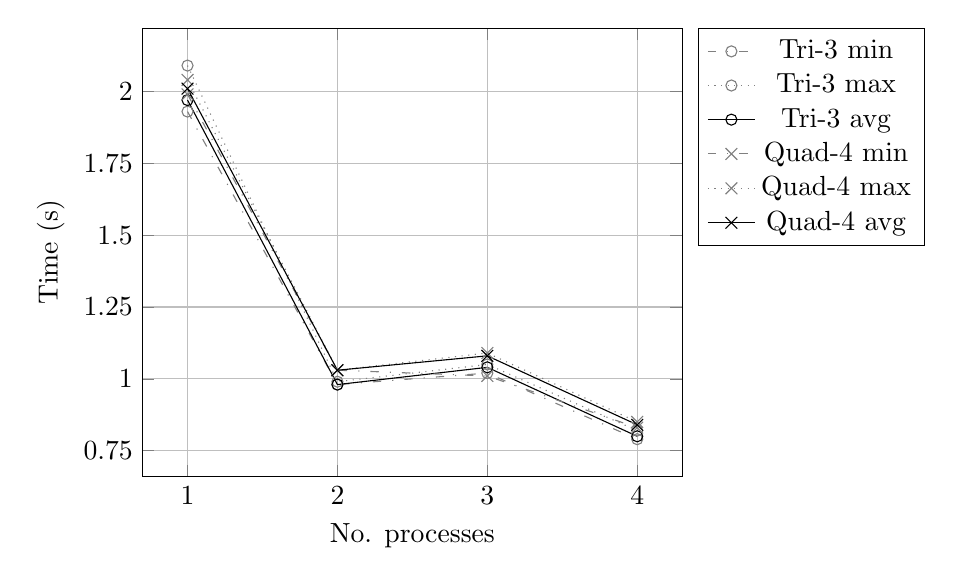
\begin{tikzpicture}
   	\begin{axis}[xlabel=No. processes,
   	ylabel=Time (s),
   	xtick={1,2,3,4},
   	ytick={2,1.75,1.5,1.25,1,0.75},
   	grid=major,
   	legend pos=outer north east]
   	\addplot[mark=o,loosely dashdotted,gray,mark options={solid}] plot coordinates {
   		(1,1.93)
   		(2,0.98)
   		(3,1.02)
   		(4,0.79)
   	};  
   	\addlegendentry{Tri-3 min}
   	\addplot[mark=o,dotted,gray,mark options={solid}] plot coordinates {
   		(1,2.09)
   		(2,0.99)
   		(3,1.05)
   		(4,0.82)
   	};  
   	\addlegendentry{Tri-3 max}
   	\addplot[mark=o,black] plot coordinates {
   		(1,1.97)
   		(2,0.98)
   		(3,1.04)
   		(4,0.8)
   	};  
   	\addlegendentry{Tri-3 avg}
   	%%%%%%%%%%%%%%%%%%%%%%%%%%%%%%%%%%%%%%%%%%%%%%%%%%%%%%%%%	
   	\addplot[mark=x,loosely dashdotted,gray,mark options={scale=1.5,solid}] plot coordinates {
   		(1,1.99)
   		(2,1.03)
   		(3,1.01)
   		(4,0.83)
   	};
   	\addlegendentry{Quad-4 min}
   	\addplot[mark=x,dotted,gray,mark options={scale=1.5,solid}] plot coordinates {
   		(1,2.04)
   		(2,1.03)
   		(3,1.09)
   		(4,0.85)
   	};
   	\addlegendentry{Quad-4 max}
   	\addplot[mark=x,black,mark options={scale=1.5}] plot coordinates {
   		(1,2.01)
   		(2,1.03)
   		(3,1.08)
   		(4,0.84)
   	};
   	\addlegendentry{Quad-4 avg}
   	\end{axis}
   	\end{tikzpicture}
   	\caption{Assembly Times}
   	\label{fig:assembly-times}
   \end{figure}
   
   \begin{figure}[htbp]
   	\centering
   	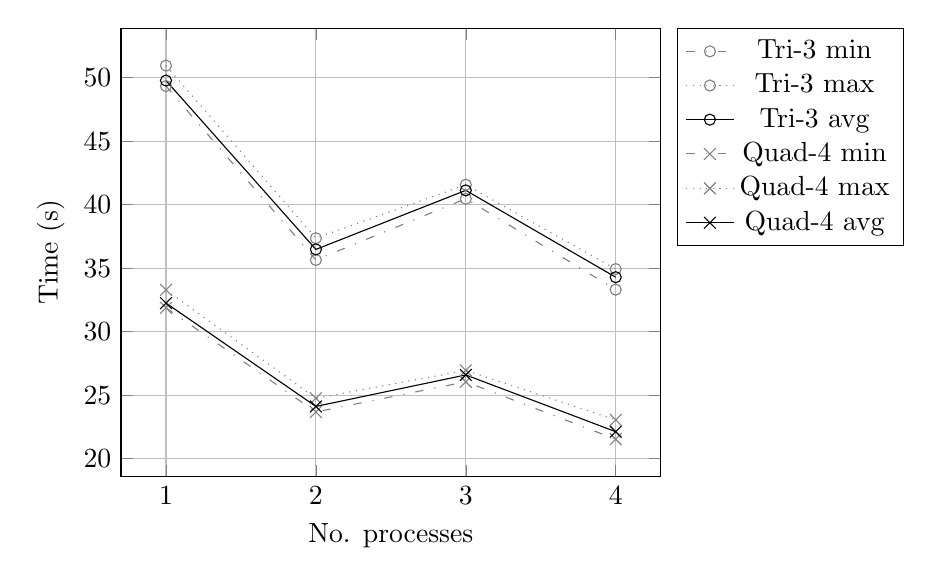
\begin{tikzpicture}
   	\begin{axis}[xlabel=No. processes,
   	ylabel=Time (s),
   	xtick={1,2,3,4},
   	ytick={50,45,40,35,30,25,20},
   	grid=major,
   	legend pos=outer north east]
   	\addplot[mark=o,loosely dashdotted,gray,mark options={solid}] plot coordinates {
   		(1,49.35)
   		(2,35.65)
   		(3,40.47)
   		(4,33.31)
   	};  
   	\addlegendentry{Tri-3 min}
   	\addplot[mark=o,dotted,gray,mark options={solid}] plot coordinates {
   		(1,50.96)
   		(2,37.36)
   		(3,41.57)
   		(4,34.93)
   	};  
   	\addlegendentry{Tri-3 max}
   	\addplot[mark=o,black] plot coordinates {
   		(1,49.78)
   		(2,36.48)
   		(3,41.13)
   		(4,34.29)
   	};  
   	\addlegendentry{Tri-3 avg}
   	%%%%%%%%%%%%%%%%%%%%%%%%%%%%%%%%%%%%%%%%%%%%%%%%%%%%%%%%%	
   	\addplot[mark=x,loosely dashdotted,gray,mark options={scale=1.5,solid}] plot coordinates {
   		(1,31.88)
   		(2,23.67)
   		(3,26.05)
   		(4,21.53)
   	};
   	\addlegendentry{Quad-4 min}
   	\addplot[mark=x,dotted,gray,mark options={scale=1.5,solid}] plot coordinates {
   		(1,33.29)
   		(2,24.75)
   		(3,26.95)
   		(4,23.05)
   	};
   	\addlegendentry{Quad-4 max}
   	\addplot[mark=x,black,mark options={scale=1.5}] plot coordinates {
   		(1,32.25)
   		(2,24.11)
   		(3,26.59)
   		(4,22.12)
   	};
   	\addlegendentry{Quad-4 avg}
   	\end{axis}
   	\end{tikzpicture}
   	\caption{Solver Times}
   	\label{fig:solver-times}
   \end{figure}
   
   \begin{figure}[htbp]
   	\centering
   	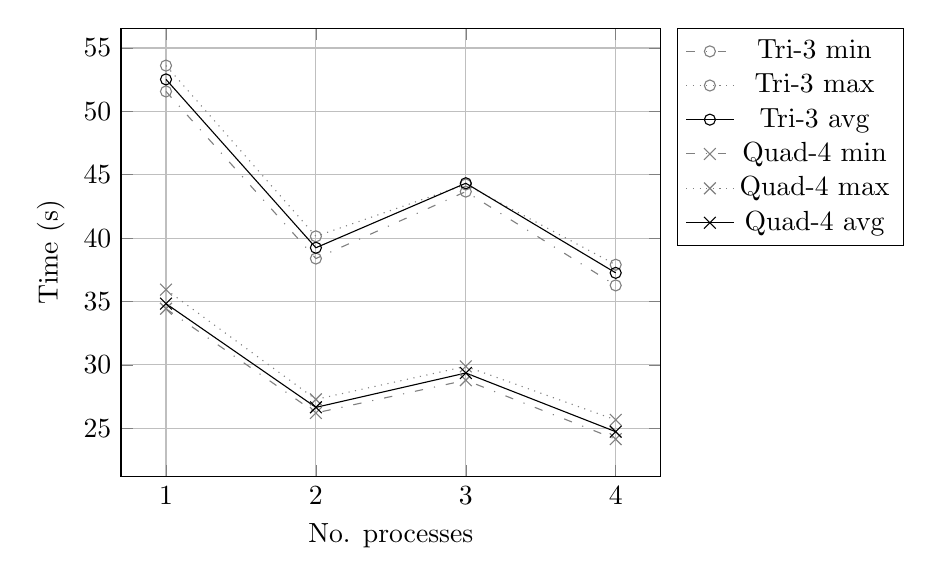
\begin{tikzpicture}
   	\begin{axis}[xlabel=No. processes,
   	ylabel=Time (s),
   	xtick={1,2,3,4},
   	ytick={55,50,45,40,35,30,25},
   	grid=major,
   	legend pos=outer north east]
   	\addplot[mark=o,loosely dashdotted,gray,mark options={solid}] plot coordinates {
   		(1,51.57)
   		(2,38.39)
   		(3,43.67)
   		(4,36.27)
   	};  
   	\addlegendentry{Tri-3 min}
   	\addplot[mark=o,dotted,gray,mark options={solid}] plot coordinates {
   		(1,53.61)
   		(2,40.14)
   		(3,44.23)
   		(4,37.90)
   	};  
   	\addlegendentry{Tri-3 max}
   	\addplot[mark=o,black] plot coordinates {
   		(1,52.52)
   		(2,39.24)
   		(3,44.33)
   		(4,37.26)
   	};  
   	\addlegendentry{Tri-3 avg}
   	%%%%%%%%%%%%%%%%%%%%%%%%%%%%%%%%%%%%%%%%%%%%%%%%%%%%%%%%%	
   	\addplot[mark=x,loosely dashdotted,gray,mark options={scale=1.5,solid}] plot coordinates {
   		(1,34.43)
   		(2,26.21)
   		(3,28.79)
   		(4,24.14)
   	};
   	\addlegendentry{Quad-4 min}
   	\addplot[mark=x,dotted,gray,mark options={scale=1.5,solid}] plot coordinates {
   		(1,35.94)
   		(2,27.28)
   		(3,29.88)
   		(4,25.66)
   	};
   	\addlegendentry{Quad-4 max}
   	\addplot[mark=x,black,mark options={scale=1.5}] plot coordinates {
   		(1,34.83)
   		(2,26.65)
   		(3,29.36)
   		(4,24.73)
   	};
   	\addlegendentry{Quad-4 avg}
   	\end{axis}
   	\end{tikzpicture}
   	\caption{Overall Times}
   	\label{fig:overall-times}
   \end{figure}
   
 %TODO satz auf halde: A fluid-structure interaction simulation with a real-world fluid solver is still in progress at the time this thesis was completed.
 \subsection{Test H: Coupled ``Bending Tower'' with fluid solver dummy}\label{sec:valid-H}
  In order to validate the coupling functionality, the developed program was tested in a coupled simulation. In order to keep the simulation for this validation simple, a fluid solver dummy was used. Its pressure values results from simple algebraic and trigonometric functions applied to the different mesh nodes. The example is based on a ``bending tower'' problem, i.e. a simple channel flow around a tower-like obstacle is simulated. The test is performed two times: First with single-threaded participants and the then again with parallelized solvers (2 processes for each solver). The setting of the test is displayed in Figure \ref{fig:testHa0}. The mesh is composed of Tri-3 elements with $\boxslash$-orientation and 2 divided square elements in x-direction and 20 divided square elements in z-direction. The coupling interface between the two solvers are the left, top and right border of the tower structure, i.e. 43 nodes (21 at every long side and one at the tip of the tower). At edge \textbf{a} the fluid solver dummy produces forces $\vec{f}_{a_i}$ for node $i$ as follows:
  \begin{equation*}
  \vec{f}_{a_i} = \begin{pmatrix}
  f_x \\ f_z
  \end{pmatrix} =
  \begin{pmatrix}
  1 + \cos\left(\frac{\tau}{25}\right) \\ 0
  \end{pmatrix}
  \end{equation*}
  for $0 \leq i \leq 20$. The $\tau$-parameter denotes the current simulation time step: $0 \leq \tau \leq 399)$. Since this example is reduced to two dimensions, only forces in x- and z-direction are present, as well as displacements $u$ and $w$. The forces are applied to the 21 nodes of edge \textbf{a}. At the top and right edge no forces are applied to their nodes.
  
  \begin{figure}[htbp]
    	\centering
    	\setlength\unitlength{1.0cm}
    	\begin{picture}(7,4)
    	\thicklines
    	\put(0.3,0.3){\vector(1,0){6.5}}\put(6.9,0.2){$x$}
    	\put(0.3,0.3){\vector(0,1){3.5}}\put(0.2,3.9){$z$}
    	\thicklines
    	\polyline(4.5,0.3)(4.5,3.3)(4.9,3.3)(4.9,0.3)  	
    	\thinlines
    	\polygon(4.5,0.3)(4.4,0.2)(4.6,0.2)\polygon(4.9,0.3)(4.8,0.2)(5,0.2)
    	
    	{\scriptsize \put(0,3.1){$2$}
    		\put(0.05,0.05){$0$}
    		\put(4.4,-0.1){$3$}\put(4.8,-0.1){$3.25$}
    		\put(4.2,1.7){$a$}}
    	\end{picture}
    	\caption{Sketch of the ``Bending Tower'' example. The rectangular structure has simply supported boundary conditions at its bottom edge. On the nodes at edge $a$ forces from the fluid solver dummy are applied, letting the tower lean forth and back during the simulation.}
    	\label{fig:testHa0}
    \end{figure}
    \begin{itemize}
     \item \textbf{Mesh dimensions}\\
     Tower height $h_t = 2$\\
     Tower length $l_t = 0.25$\\
     Tower thickness $t = 0.01$  	
      	
     \item \textbf{Material properties}\\
     Young's Modulus $E = 1.0 \times 10^8$\\
     Poisson's ratio $\nu = 0.3$
      	
     \item \textbf{Boundary conditions}\\
     The bottom side of the tower is simply supported.
     
     \item \textbf{Simulation settings}\\
     Time step length $dt = 0.01$\\
     Simulation time $time = 4.0$\\
     Time steps $\tau_{max} = 400$\\
     preCICE coupling-scheme: serial-implicit\\
     preCICE mapping-scheme: Nearest-Neighbor
    \end{itemize}
    \paragraph{Results:} The coupling finished successfully after 400 simulated time steps without errors. The analysis of the calculated displacements during the simulation showed the intended behavior, as can be seen in Figure \ref{fig:testHa1} for the two displacements $u$ in x- and $w$ in z-direction. In Figure \ref{fig:testHa2} the deformed mesh at different time steps are presented, visualizing the bending of the tower. Although this test was performed with a non-physical fluid solver, the coupling itself between two different and independent solvers via preCICE was successful. In this test, both participants were executed in serial as well as in parallel (2 processes for each solver). Both simulations reached their end successfully and showed the same results.

	\begin{figure}[htbp]
	 \centering
	 \includegraphics[width=1.0\linewidth]{figures/i-beam_w}
     \caption{The displacements $u$ in x- and $w$ in z-direction for the topmost node of the left edge is plotted over time. The smooth oscillating behavior of the tower that was intended in the test is clearly visible. The motion in x-direction is larger due to the forces facing the same direction.}
	 \label{fig:testHa1}
	\end{figure}    

    \begin{landscape}
     \begin{figure}[htbp]
      \centering
      \includegraphics[width=0.8\linewidth]{figures/frames}
      \caption{Single time steps of the bending tower test. A rainbow color gradient shows the absolute displacements in z-direction, with red being maximal positive, green equals zero and blue being maximal negative. At time step 1, the tip of the structure is already moving towards the positive x-axis, since the initial force applied to the left side is $1$. Time step 118 shows the reversal point (no force) at the left side and time step 197 shows the other reversal point of the tower during the simulation where the force is maximal with a value of $2$.}
      \label{fig:testHa2}
     \end{figure}
    \end{landscape}
  
 \subsection{Test I: Coupled ``Bending Tower'' with fluid solver}\label{sec:valid-I}
  The developed program is tested in a fluid-structure interaction. In the simulation the program is coupled with a fluid solver developed with OpenFOAM, an open-source software for computational fluid dynamics \cite{openfoam-url}. % from . at Delft 
  As example problem, a simple channel flow around a tower-like obstacle is simulated. The geometry configuration can be seen in Figure \ref{fig:testI0}. The fluid solver simulates the flow coming in from the left edge of the channel and moving towards the right edge, where the flow leaves the fluid domain. The tower is placed at the bottom side of the channel and has simply supported boundary conditions at its bottom edge. The tower structure is simulated by the thesis' program. The coupling interface region in this test is the left, top and right border of the tower. When the flow reaches the left side of the tower, it will bend to the right side due to the forces steadily increasing by the flow. After some time the tower will not bend further to the right, when an equilibrium of forces between the tower and the flow is reached.
  
  \begin{figure}[htbp]
  	\centering
  	\setlength\unitlength{1.0cm}
  	\begin{picture}(11,4)
  	\thicklines
  	\put(0.3,0.3){\vector(1,0){10.5}}\put(10.9,0.2){$x$}
  	\put(0.3,0.3){\vector(0,1){3.5}}\put(0.2,3.9){$y$}
  	\linethickness{0.5mm}
  	\polygon(0.3,0.3)(0.3,3)(10.3,3)(10.3,0.3)
  	\thicklines
  	\polyline(3.3,0.3)(3.3,1.634)(3.8,1.634)(3.8,0.3)  	
  	\thinlines
  	\polygon(3.3,0.3)(3.15,0.15)(3.45,0.15)\polygon(3.8,0.3)(3.65,0.15)(3.95,0.15)
  	\multiput(0.5,0.6)(0,0.5){5}{\vector(1,0){0.5}}
  	\multiput(9.6,0.6)(0,0.5){5}{\vector(1,0){0.5}}
  	\multiput(3.3,0.6)(0,0.3){3}{\line(1,-1){0.5}} %balken schraffieren
  	
  	{\scriptsize \put(0,2.9){$4$}\put(0,1.53){$2$}
  		\put(0.05,0.05){$0$}
  		\put(3.2,-0.14){$3$}\put(3.72,-0.14){$3.5$}\put(10.12,-0.14){$10$}}
  	\end{picture}
  	\caption{Sketch of the ``Bending Tower'' example. An rectangular obstacle is put into a channel and flow is driven from the left side towards the right side where it leaves the fluid domain. The tower-like obstacle is represented by the structure mesh, the channel by the fluid mesh.}
  	\label{fig:testI0}
  \end{figure}
  %TODO discretization of the tower mesh + fluid mesh
  %TODO                                                                                                                            yy                         yy
  The tower mesh consists of $4\!\times\!8$ Quad-4 elements (4 elements in x-, 8 in y-direction). The fluid domain is divided into XX cells on the x-axis and xx cells on the y-axis. The coupling surface is at the left, right and top border of the structure mesh, resulting in 18 nodes for both participants.
  
  \begin{itemize}
  	\item \textbf{Mesh dimensions}\\
  	Tower height $h_t = 2$\\
  	Tower length $l_t = 0.5$\\
  	Tower thickness $t = 0.1$\\
  	Channel height $h_c = 4$\\
  	Channel length $l_c = 10$  	
  	
  	\item \textbf{Material properties}\\
  	Young's Modulus $E = 1.0 \times 10^9$\\
  	Poisson's ratio $\nu = 0.3$
  	
  	%TODO add preCICE information
  	\item \textbf{preCICE setup}\\
    Maximum time step length $0.1$\\
    Coupling-scheme: serial-implicit\\
    Mapping-scheme: Nearest-Neighbor
  	
  	%TODO add FOAM-FSI information
  	\item \textbf{fluid solver setup}\\
    Simulation time $time = 8.0$\\
    Time step length $\delta T = 0.002$\\
  	Initial flow velocity in x-direction: $0.001$\\
  	Inlet flow velocity: Ramped-up inlet with maximum value of $0.2$\\
  	
  	\item \textbf{Boundary conditions}\\
  	The bottom side of the tower is simply supported.
  	The top and bottom side of the channel is %TODO....gleitbedingungen/haftbedingungen
  \end{itemize}
  
  \paragraph{Results:} 
   Figure \ref{fig:testI1} shows single time steps of the simulation. One can see the interaction between the fluid and structure by the motion of the tower and the reaction of the flow velocity around it. In Figure \ref{fig:testI2} the flow velocity at the topmost right node of the coupling interface region is plotted over time. Here, one can see the reaction of the flow to the contact with the tower, too. %TODO
  %TODO bild von u/v over time plotted
  \begin{figure}[htbp]
   \label{fig:testI2}
   \centering
   \includegraphics[width=0.8\linewidth]{figure/fsi_uw}
   \caption{}
  \end{figure}
  
  %TODO bild von verschiedenen timesteps
  \begin{landscape}
   \begin{figure}
    \label{fig:testI1}
    \centering
    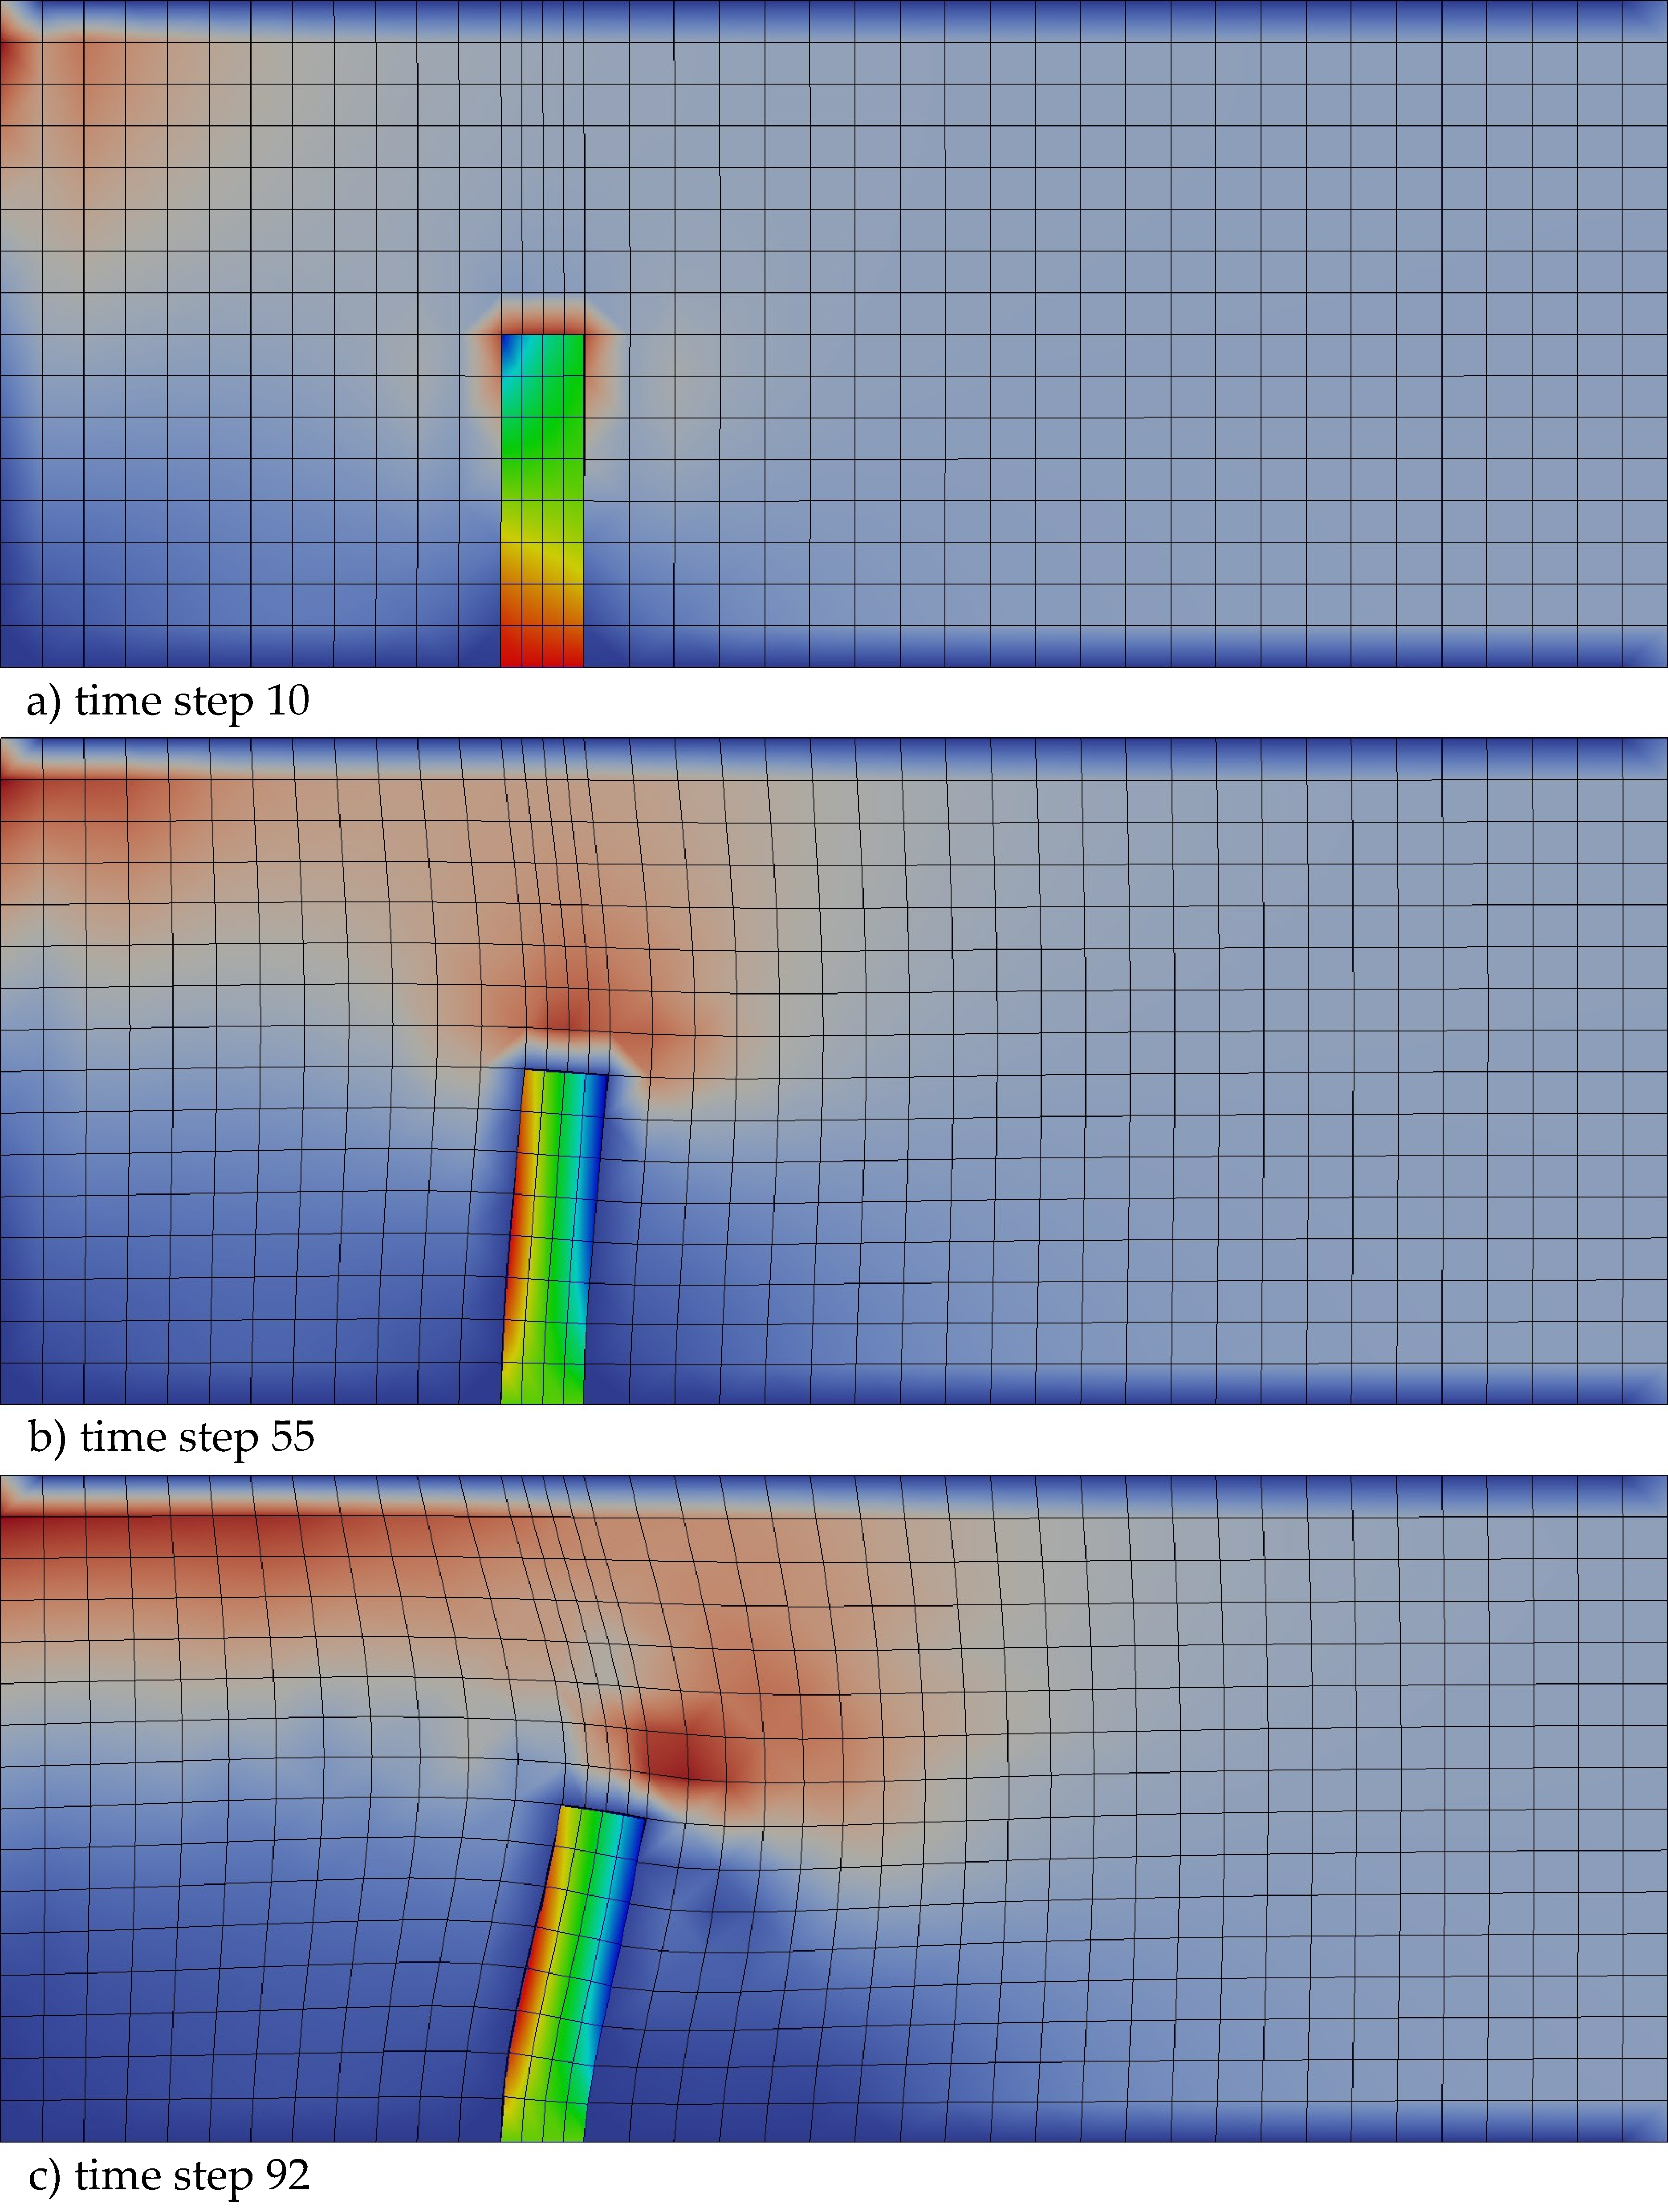
\includegraphics[width=0.75\linewidth]{figure/fsi_frames}
    \caption{}
   \end{figure}
  \end{landscape}

\section{Summary and Conclusions}
 This chapter summarizes the important results achieved by the thesis and presents a discussion of these results. In the remainder of this chapter an outlook to future development is given.
 
 
 \subsection{Summary}
 % was war das ziel
  The aim of the thesis was to develop a FEM-code being able to be coupled in a fluid-structure interaction. The program development should be supported by a FEM framework. Comparison aspects had to be created and an evaluation of several FEM libraries was performed. The implemented FEM-code was to be validated with example problems. The coupling part should be managed by the preCICE tool. The overall focus was on creating a well documented and easily readable and maintainable code, ready for further development and extensions.
  
  For the FEM framework evaluation different comparison aspects were introduced. Besides organizational requirements like an open-source code, C++ as development programming language and a wide and accurate documentation of the functions and classes, numerical and programmatic aspects were considered. The last aspects included the possibility to parallelize the code via MPI, a large collection of finite element types and built-in iterative linear solvers. During the evaluation process two libraries were practically tested, the first one being MFEM. Because of difficulties in use, another library - libMesh - was tested and finally chosen for the program development.
  
  In this thesis flat shell elements were implemented. Such an element is composed of a plane and a plate element part that are superimposed in order to construct the final shell element. Two different types of finite elements were considered: A three-node triangular element, denoted as Tri-3 and a four-node quadrilateral element, denoted as Quad-4. Six models had to be implemented in the scope of this thesis: A plane, plate and shell element for each of the two discretizations. Therefore, existing models like the Discrete Kirchhoff Quadrilateral were taken.
  %...
  
  % implementation
  
  % validation

 % was wurde gemacht, im prinzip introduction nur in vergangenheitsform
 % keine schlussfolgerungen! das kommt er im nächsten abschnitt
 
 \subsection{Conclusion}
 % dieser teil sollte lang sein
 % es wurden verschiedene frameworks mit einander verglichen und das geignetste ausgewählt. MFEM und libMesh waren in der näheren auswahl. libMesh ist nachträglich betrachtet tatsächlich eine gute wahl gewesen. vorher wurde probiert mit MFEM zu arbeiten, aber gewisse probleme haben einen wechsel provoziert.
 % es wurden 6 finite elemente implementiert und getestet. das war nötig um einen geiegneten strukturlöser für die kopplung zu haben.
 % die einzelnen tests (nochmal) analysieren (accuracy, etc.)
 % test der convergence
 % test der parallelität
 % test der kopplung
 
 % resumé: löser geeignet für multi-physics, wenn unterteilung des meshs entsprechend hoch ist, damit accuracy stimmt. dank gut skalierender parallelisierung möglich 

 \subsection{Future Development}
  The developed FEM-code successfully implemented flat shell elements and is able to work in coupled multi-physics simulations. The validation showed good accuracy for fine mesh subdivisions. The program was designed to be able to easily introduce new models for plane and plate elements, for example quadratic or cubic quadrilateral elements with 8 or 9 nodes. This would enhance the accuracy further. The requirements of the developed program included two dimensional elements. One could expand this limit also to beam and truss elements of one dimension or even to three dimensional solid elements. The libMesh library and the coupling tool preCICE would support such features.
  
  All scenarios considered in this work so far had constant conditions. The finite element idealization could be extended to situations that are time dependent and simultaneously add dynamic behavior to the elastic structures. When displacements of an elastic body vary with time two additional forces must be introduced, namely the inertia or acceleration and resistance opposing the motion. Therefore, a new type of solver must be introduced as well which might also be provided by the libMesh framework.
\newpage

\bibliographystyle{alpha}
\bibliography{thesis}

\Affirmation
\end{document}